
\section{Implementation: Anykernel and Rump Kernels}
\label{chap:implementation}

The previous chapter discussed the concept of an anykernel and rump
kernels.  This chapter describes the code level modifications that
were necessary for a production quality implementation on NetBSD.
The terminology used in this chapter is mainly that of NetBSD, but the
concepts apply to other similar operating systems as well.

In this chapter we reduce the number of variables in the discussion by
limiting our examination to rump kernels and their clients running on a
NetBSD host.  See the next chapter (\chapref{ecosystem}) for discussion on
rump kernels and their clients running on hosts beyond NetBSD userspace.


\subsection{Kernel Partitioning}
\label{sect:partition}

As mentioned in Section~\ref{sect:conceptintro}, to maximize the
lightweight nature of rump kernels, the kernel code was several
logical layers: a base, three factions (dev, net and vfs) and drivers.
The factions are orthogonal, meaning they do not depend on each other.
Furthermore, the base does not depend on any other part of the kernel.
The modifications we made to reach this goal of independence are described
in this section.

As background, it is necessary to recall how the NetBSD kernel is linked.
In C linkage, symbols which are unresolved at compile-time must be
satisfied at binary link-time.  For example, if a routine in
\texttt{file1.c} wants to call \texttt{myfunc()} and \texttt{myfunc()}
is not present in any of the object files or libraries being linked
into a binary, the linker flags an error.  A monolithic kernel
works in a similar fashion:  all symbols must be resolved when the
kernel is linked.  For example, if an object file with an unresolved
symbol to the kernel's pathname lookup routine \texttt{namei()} is
included, then either the symbol \verb+namei+ must be provided by
another object file being linked, or the calling source module must
be adjusted to avoid the call.  Both approaches are useful for us
and the choice depends on the context.

We identified three obstacles for having a partitioned kernel:

\begin{enumerate}
\item   \textbf{Compile-time definitions} (\texttt{\#ifdef}) indicating
	which features are present in the kernel.  Compile-time
	definitions are fine within a component, but do not work
	between components if linkage dependencies are created
	(for example a cross-component call which is conditionally
	included in the compilation).

\item   \textbf{Direct references} between components where we do
	not allow them.  An example is a reference from the base
	to a faction.

\item   \textbf{Multiclass source modules} contain code which
	logically belongs in several components.  For example, if
	the same file contains routines related to both file systems
	and networking, it belongs in this problem category.
\end{enumerate}

Since our goal is to change the original monolithic kernel and its
characteristics as little as possible, we wanted to avoid heavy
approaches in addressing the above problems.  These approaches
include but are not limited to converting interfaces to be called only
via pointer indirection.  Instead, we observed that indirect
interfaces were already used on most boundaries (\eg \texttt{struct
fileops}, \texttt{struct protosw}, etc.) and we could concentrate
on the exceptions.  Code was divided into functionality groups
using source modules as boundaries.

The two techniques we used to address problems are as follows:

\begin{enumerate}
\item   \textbf{code moving}.  This solved cases where a source
	module belonged to several classes.  Part of the code was
	moved to another module.  This technique had to be used
	sparingly since it is very intrusive toward other developers
	who have outstanding changes in their local trees.  However,
	we preferred moving over splitting a file into several
	portions using \texttt{\#ifdef}, as the final result is
	clearer to anyone looking at the source tree.

	In some cases code, moving had positive effects beyond rump
	kernels.  One such example was splitting up
	\verb+sys/kern/init_sysctl.c+, which had evolved to include
	\textit{sysctl} handlers for many different pieces of
	functionality.  For example, it contained the routines
	necessary to retrieve a process listing.  Moving the process
	listing routines to the source file dealing with process
	management (\verb+sys/kern/kern_proc.c+) not only solved
	problems with references to factions, but also
	grouped related code and made it easier to locate.

\item   \textbf{function pointers}.  Converting direct references
	to calls via function pointers removes link-time restrictions.
	A function pointer gets a default value at compile time.
	Usually this value is a stub indicating the requested feature is
	not present.  At runtime the pointer may be adjusted to
	point to an actual implementation of the feature if it is
	present.
\end{enumerate}

Previously, we also used weak symbol aliases sparingly to provide stub
implementations which were overridden by the linker if the component
providing the actual implementation was linked.  Weak aliases were
found to be problematic with dynamically linked libraries on some
userspace platforms, \eg Linux with glibc.  In \textit{lazy binding},
a function is resolved by the dynamic linker only when the function
is first called, so as to avoid long program startup times due to resolving
symbols which are never used at runtime.  As a side-effect, lazy binding
theoretically allows \texttt{dlopen()}'ing libraries which override weak
aliases as long as the libraries are loaded before the overridden functions
are first called.  Namely, in the case of rump kernels, loading must
take place before \verb+rump_init()+ is called.  However, some dynamic
linkers treat libraries loaded with \texttt{dlopen()} different from
ones loaded when the binary is executed.  For example, the aforementioned
glibc dynamic linker overrides weak aliases with symbols from
\texttt{dlopen()}'d libraries only if the environment variable
\verb+LD_DYNAMIC_WEAK+ is set.  With some other dynamic linkers,
overriding weak symbols is not possible at all.  Part of the power of
rump kernels is the ability to provide a single binary which dynamically
loads the necessary components at runtime depending on the configuration
or command line parameters.  Therefore, to ensure that rump kernels work
the same on all userspace platforms, we took the extra steps necessary
to remove uses of weak aliases and replace them with the above-mentioned
two techniques.

To illustrate the problems and our necessary techniques, we discuss
the modifications to the file \verb+sys/kern/kern_module.c+.  The
source module in question provides support for loadable kernel
modules (discussed further in Section~\ref{sect:extending}).
Originally, the file contained routines both for loading kernel
modules from the file system and for keeping track of them.  Having
both in one module was a valid possibility before the anykernel faction
model.  In the anykernel model, loading modules from a file system is VFS
functionality, while keeping track of the modules is base functionality.

To make the code comply with the anykernel model, we used the code
moving technique to move all code related to file system access to
its own source file in \verb+kern_module_vfs.c+.  Since loading from
a file system must still be initiated by the kernel module management
routines, we introduced a function pointer interface.  By default,
it is initialized to a stub:

{\small
\begin{verbatim}
int (*module_load_vfs_vec)(const char *, int, bool, module_t *,
                           prop_dictionary_t *) = (void *)eopnotsupp; 
\end{verbatim}}

If VFS is present, the routine \verb+module_load_vfs_init()+ is
called during VFS subsystem init after the \verb+vfs_mountroot()+
routine has successfully completed to set the value of the function
pointer to \verb+module_load_vfs()+.  In addition to avoiding a
direct reference from the base to a faction in rump kernels, this
pointer has another benefit: during bootstrap it protects the kernel from
accidentally trying to load kernel modules from the file system before
the root file system has been mounted~\footnote{\texttt{sys/kern/vfs\_subr.c}
rev 1.401}.

\subsubsection{Extracting and Implementing}

We have two methods for providing functionality in the rump kernel:
we can \textit{extract} it out of the kernel sources, meaning we
use the source file as such, or we can \textit{implement}
it, meaning that we do an implementation suitable for use in a rump
kernel.  We work on a source file granularity level, which means
that either all of an existing source file is extracted, or the
necessary routines from it (which may be all of them) are implemented.
Implemented source files are placed under \texttt{sys/rump},
while extracted ones are picked up by Makefiles from other subdirectories
under \texttt{sys/}.

The goal is to extract as much as possible for the features
we desire, as to minimize implementation and maintenance effort and to
maximize the semantic correctness of the used code.  Broadly speaking,
there are three cases where extraction is not possible.

\begin{enumerate}
\item   \textbf{code that does not exist in the regular kernel}: this
	means drivers specific to rump kernels.  Examples include
	anything using rump hypercalls, such as the virtual
	block device driver.

\item	\textbf{code dealing with concepts not supported in
	rump kernels}.  An example is the virtual memory fault handler:
	when it is necessary to call a routine which in a regular
	kernel is invoked from the fault hander, it must be done from
	implemented code.

        It should be noted, though, that not all VM code should
        automatically be disqualified from extraction.  For instance,
        VM readahead code is an algorithm which does not have anything
        per se to do with virtual memory, and we have extracted it from
	\verb+sys/uvm/uvm_readahead.c+.

\item   \textbf{bypassed layers} such as scheduling.  They need
	different handling.
\end{enumerate}

In some cases a source module contained code which was desirable to be
extracted, but it was not possible to use the whole source module
because others parts were not suitable for extraction.  Here we
applied the code moving technique.  As an example, we once again
look at the code dealing with processes (\verb+kern_proc.c+).
The source module contained mostly process data structure management routines,
\eg the routine for mapping a process ID number (\verb+pid_t+) to the structure
describing it (\texttt{struct~proc~*}).  We were interested in being
able to extract this code.  However, the same file also contained the
definition of the \texttt{lwp0} variable.  Since that definition
included references to the scheduler (``concept not supported in
a rump kernel''), we could not extract the file as such.  However,
after moving the definition of \texttt{lwp0} to \verb+kern_lwp.c+,
where it arguably belongs, \verb+kern_proc.c+ could be extracted.


\subsubsection{Providing Components}
\label{sect:components}

We provide components as libraries.
The kernel base library is called \texttt{librump} and
the hypervisor library is called \texttt{librumpuser}.  The factions
are installed with the names \texttt{librumpdev}, \texttt{librumpnet}
and \texttt{librumpvfs} for dev, net and vfs, respectively.  The
driver components are named with the pattern
\verb+librump<faction>_driver+, \eg \verb+librumpfs_nfs+ (NFS client
driver).  The faction part of the name is an indication of what
type of driver is in question, but it does not convey definitive
information on what the driver's dependencies are.  For example,
consider the NFS client: while it is a file system driver, it
also depends on networking.

\begin{figure}[t]
\includegraphics{imgs/sharedstatic}
\caption[Performance of position independent code (PIC)]
{\textbf{Performance of position independent code (PIC).}
A regular kernel is compiled as non-PIC code.  This compilation
mode is effectively the same as ``none'' in the graph.  If the hypervisor
and rump kernel base use PIC code, the execution time increases as
is expected.  In other words, rump kernels allow to make a decision on
the tradeoff between execution speed and memory use.
}
\label{fig:sharedstatic}
\end{figure}

Two types of libraries are available: static and dynamic.  Static
libraries are linked by the toolchain into the binary, while dynamic
binaries are linked at runtime.  Commonly, dynamic linking is used
with shared libraries compiled as position independent code (PIC), so as
to allow one copy of a library to be resident in memory and be mapped
into an arbitrary number of programs.  Rump kernels support both types
of libraries, but it needs to be noted that dynamic linking depends on
the host supporting that runtime feature.  It also need to be noted
that while shared libraries save memory in case they are needed more
than once, they have inherently worse performance
due to indirection~\cite{gingell:shlib}.
Figure~\ref{fig:sharedstatic} illustrates that performance penalty by
measuring the time it takes to create and disband 300k threads in a
rump kernel.  As can be deduced from the combinations, shared and static
libraries can be mixed in a single rump kernel instance so as to further
optimize the behavior with the memory/CPU tradeoff.

\subsection{Running the Kernel in an Hosted Environment}

Software always runs on top of an entity which provides the interfaces
necessary for the software to run.  A typical operating system
kernel runs on top of hardware and uses the hardware's ``interfaces''
to fulfill its needs.  When running on top a hardware emulator the
emulator provides the same hardware interfaces.  In a paravirtualized
setup the hypervisor provides the necessary interfaces.  In a
usermode OS setup, the application environment of the hosting OS
makes up the hypervisor.  In this section we discuss details related
to hosting a rump kernel in any environment.  We use POSIX
userspace as the case for the bulk of the discussion, since that host induces
the superset of issues related to hosting rump kernels.

\subsubsection{C Symbol Namespaces}
\label{chap:rumpns}

In the regular case, the kernel and userspace C namespaces are disjoint.
Both the kernel and application can contain the same symbol name,
for example \texttt{printf}, without a collision occurring.  When we
run the kernel in a process container, we must take care to preserve
this property.  Calls to printf made by the client still need to go to
libc, while calls to printf made by the rump kernel need to be handled by
the in-kernel implementation.

Single address space operating systems provide a
solution~\cite{deller:sasoslink}, but require a different calling
convention.  On the other hand, C preprocessor macros were used by
OSKit~\cite{ford:oskit} to rename conflicting symbols and allow multiple
different namespaces to be linked together.  UML~\cite{dike:uml}
uses a variant of the same technique and renames colliding symbols
using a set of preprocessor macros in the kernel build Makefile,
\eg \verb+-Dsigprocmask=kernel_sigprocmask+.  This manual renaming
approach is inadequate for a rump kernel; unlike a usermode OS kernel
which is an executable application, a rump kernel is a library which is
compiled, shipped, and may be linked with any other libraries afterwards.
This set of libraries is not available at compile time and therefore we
cannot know which symbols will cause conflicts at link time.  Therefore,
the only option is to assume that any symbol may cause a conflict.

We address the issue by protecting all symbols within the rump
kernel.  The \texttt{objcopy} utility's rename functionality is
used ensure that all symbols within the rump kernel have a prefix
starting with ``rump'' or ``RUMP''.  Symbol names which do not
begin with ``rump'' or ``RUMP''
are renamed to contain the prefix ``rumpns\_''.  After
renaming, the kernel \texttt{printf} symbol will be seen as
\texttt{rumpns\_printf} by the linker.  Prefixes are illustrated
in Figure~\ref{fig:namespace}: callers outside of a rump kernel
must include the prefix explicitly, while the prefix for routines
inside a rump kernel is implicit since it is automatically added
by \texttt{objcopy}.  Table~\ref{tab:symren} illustrates further
by providing examples of the outcome of renaming.

However, renaming all symbols also creates a problem.  Not all
symbols in a kernel object file come from kernel source code.
Some symbols are a property of the toolchain.  An example is
\verb+_GLOBAL_OFFSET_TABLE_+, which is used by position independent
code to store the offsets.  Renaming toolchain-generated symbols
causes failures, since the toolchain expects to find symbols where
it left them.

\begin{figure}[t]
\begin{center}
\includegraphics[width=5.3cm,height=3cm]{imgs/vpk_namespace}
\caption[C namespace protection]{\textbf{C namespace protection}.  When
referencing a rump kernel symbol from outside of the rump kernel, the
prefix must be explicitly included in the code.  All references from
inside the rump kernel implicitly contain the prefix due to bulk
symbol renaming.  Corollary: it is not possible to access a symbol
outside the rump kernel namespace from inside the rump kernel without
using a hypercall.}
\label{fig:namespace}
\end{center}
\end{figure}

\begin{table}[t]
\begin{tabular}{|l|l|l|}
\hline
rump kernel object & original symbol name & symbol after renaming \\
\hline
\hline
yes & \verb+rump_sys_call+ & \verb+rump_sys_call+ \\
\hline
yes & \verb+printf+ & \verb+rumpns_printf+ \\
\hline
no & \verb+rump_sys_call+ & \verb+rump_sys_call+ \\
\hline
no & \verb+printf+ & \verb+printf+ \\
\hline
\end{tabular}
\caption[Symbol renaming illustrated]{\textbf{Symbol renaming
illustrated.}  Objects belonging to a rump kernel have their exported
symbols and symbol dereferences renamed, if necessary, so that they are
inside the rump kernel namespace.  Objects which do not belong to a rump
kernel are not affected.}
\label{tab:symren}
\end{table}

We observed that almost all of the GNU toolchain's symbols are in
the double-underscore namespace ``\_\_'', whereas the NetBSD kernel
exported under 10 symbols in that namespace.  The decision was to
rename existing kernel symbols in the double underscore namespace
to a single underscore namespace and exclude the double underscore
namespace from the rename.  There were two exceptions to the double
underscore rule which had to be excluded from the rename as well:
\verb+_GLOBAL_OFFSET_TABLE_+ and architecture specific ones.
We handle the architecture specific ones with a quirk table.  There
is one quirk each for PA-RISC, MIPS, and PowerPC64.  For example,
the MIPS toolchain generates the symbol \verb+_gp_disp+, which
needs to be excluded from the renaming.  Experience of over 5
years shows that once support for an architecture is added,
no maintenance is required.

We conclude mass renaming symbols is a practical and feasible
solution for the symbol collision problem which, unlike manual
renaming, does not require knowledge of the set of symbols that
the application namespace exports.

\subsubsection{Privileged Instructions}
\label{sect:privinst}

Kernel code dealing with for example the MMU may execute CPU
instructions which are available only in privileged mode.  Executing
privileged instructions while in non-privileged mode should cause
a trap and the host OS or VMM to take control.  Typically, this trap
will result in process termination.

Virtualization and CPU emulation technologies solve the problem by
not executing privileged instructions on the host CPU in unprivileged mode.
For example, paravirtualized Xen~\cite{barham:xen} uses hypercalls, User Mode
Linux~\cite{dike:uml} does not use privileged instructions in the
usermode machine dependent code, QEMU~\cite{bellard:qemu}
handles such instructions in the machine emulator, and CPU virtualization
extensions trap the handling of those instructions to the hypervisor.

In practice kernel drivers do not use privileged instructions
because they are found only in the architecture specific parts of
the kernel.  Therefore, we can solve the problem by defining that
it does not exist in our model --- if there are any it is a failure
in modifying the OS to support rump kernels.

\subsubsection{The Hypercall Interface(s)}
\label{sect:hypercall}

The hypercall interfaces allow a rump kernel to access host platform
resources and integrate with the host.  For example, page level
memory allocation and the blocking and running of threads is
accomplished via the hypercall interface.  Essentially, the hypercall
interface represents the \textit{minimal} interface for running kernel
drivers.  As we shall see later in Section~\ref{sect:rumprun},
transitively the hypercall interface is also the minimal interface
for running POSIX applications.  Notably, the Embassies
project~\cite{howell:embassies} investigated a minimal execution
interface for applications, and ended up with a similar interface,
thereby increasing our confidence in our result being correct.

Historically, all hypercalls were globally implemented by a single
library.  This was found to be inflexible for I/O devices for two reasons:

\begin{itemize}
\item	Different I/O devices have different requirements.  Imagine
	the hypercalls for a network interface necessary to send and
	receive packets.  If you imagined a PCI network interface
	card, the necessary hypercalls are completely different from
	if you imagined \texttt{/dev/tap} or netmap~\cite{rizzo:netmap}.
	With a growing number of different I/O devices being supported,
	codifying the different requirements under a compact, fast and
	understandable interface was not seen to be reasonably possible.

\item	Not all platforms require all I/O devices to be supported.
	Globally pooling all hypercalls together obfuscates what is
	the minimal required set of hypercall functionality to run rump
	kernel on a given platform with a given set of I/O devices.
\end{itemize}

Therefore, there are now two types of hypercalls: main hypercalls,
which are always required by every rump kernel, and I/O hypercalls,
which allow given types of I/O drivers to operate.  The main hypercall
interface is a single, stable and versioned interface.  The I/O hypercalls
are private to the I/O bus or the I/O driver, and an implementation is
required only if the component using the hypercall is linked into the
rump kernel.  The versioning of I/O hypercalls and changes to them are
up to individual drivers, and for example over the course of optimizing
networking packet processing performance, we made several tweaks to the
hypercalls used by the virtual packet I/O drivers
(Section~\ref{sect:networking}).  These changes provided for example
the ability to deliver packets in bursts and zero-copy processing.
For the remainder of this section we will describe the main hypercall
interface.


\subsubsection*{Main hypercalls}

For the historical reason of rump kernels initially running in userspace,
the hypercall interface is called \textit{rumpuser}; for example
\textit{rumphyper} would be a more descriptive name, but changing it
now brings unnecessary hassle.  The version of the hypercall revision
we describe here is 17.  In reality, version 17 means the second stable
rendition of the interface, as during initial development the interface
was changed frequently and the version was bumped often.  The canonical
implementation for the interface is the POSIX platform
implementation, currently found from \texttt{lib/librumpuser} in
the NetBSD tree.  Implementations for other platforms are found from
\url{http://repo.rumpkernel.org/}, and also from 3rd parties.

As an example of a hypercall, we consider allocating memory from the host.
A hypercall is the only way that a rump kernel can allocate memory at
runtime.  Notably, though, in the fastpath case the hypercall is used
to allocate page-sized chunks of memory, which are then dosed out by
the pool and slab allocators in the rump kernel.  The signature of the memory
allocation hypercall is the following:

{\small
\begin{verbatim}
int	rumpuser_malloc(size_t howmuch, int alignment, void **retp);
\end{verbatim}}

If a hypercall can fail, its return type is \texttt{int}, and it returns
0 for success or an error code.  If a hypercall cannot fail, it is of
type \texttt{void}.  If successful, the memory allocation hypercall will have
allocated \texttt{howmuch} bytes of memory and returns a pointer to that
memory in \texttt{retp}.  The pointer is guaranteed to be aligned to
\texttt{alignment} bytes.  For example on POSIX the implementation of
this interface is a call to \verb+posix_memalign()+ or equivalent.

The header file \texttt{sys/rump/include/rump/rumpuser.h} defines the
hypercall interface.  All hypercalls by convention begin with the string
``rumpuser''.  This naming convention prevents hypercall interface
references in the rump kernel from falling under the jurisdiction of
symbol renaming and hence the hypercalls are accessible from the
rump kernel.

The hypercalls required to run rump kernels can be categorized into the
following groups:

\begin{itemize}
\item	\textbf{initialization}: bootstrap the hypercall layer and check
	that the rump kernel hypercall version matches a version
	supported by the hypercall implementation.  This interface is
	called as the first thing when a rump kernel initializes.
\item   \textbf{memory management}: allocate aligned memory, free
\item	\textbf{thread management}: create and join threads, TLS access
\item   \textbf{synchronization routines}: mutex, read/write lock,
	condition variable.
\item	\textbf{time management}: get clock value, suspend execution of
	calling thread for the specified duration
\item	\textbf{exit}: terminate the platform.  Notably, in some
	cases it is not possible to implement this fully, e.g. on
	bare metal platforms without software power control.  In that
	case, a best effort approximation should be provided.
\end{itemize}

There are also a number of optional hypercalls, which are not strictly
speaking required in all cases, but are nevertheless part of core
functionality:

\begin{itemize}
\item   \textbf{errno handling}: If system calls are to be made,
	the hypervisor must be able to set a host thread-specific
	\textit{errno} so that the client can read it.
	Note: errno handling is unnecessary if
	the clients do not use the rump system call API.
\item	\textbf{putchar}: output character onto console.  Being
	able to print console output is helpful for debugging purposes.
\item	\textbf{printf}: a printf-like call.  see discussion below.
\end{itemize}

\subsubsection*{The Benefit of a printf-like Hypercall}

The \verb+rumpuser_dprintf()+ call has the same calling convention as
the NetBSD kernel \verb+printf()+ routine.  It is used to write debug output
onto the console, or elsewhere if the implementation so chooses.
While the kernel \verb+printf()+ routine can be used to
produce debug output via \verb+rumpuser_putchar()+, the kernel
printf routine in-kernel locks to
synchronize with other in-kernel consumers of the same interface.  These
locking operations may cause the rump kernel virtual CPU context
to be relinquished, which in turn may cause inaccuracies in debug
prints especially when hunting racy bugs.  Since the hypercall runs
outside of the kernel, and will not unschedule the current rump
kernel virtual CPU, we found that debugging information produced
by it is much more accurate.  Additionally, a hypercall can be
executed without a rump kernel context.  This property was invaluable
when working on the low levels of the rump kernel itself, such as
thread management and CPU scheduling.

\subsection{Rump Kernel Entry and Exit}
\label{sect:rumpentry}

As we discussed in \chapref{concept}, a client must possess
an execution context before it can successfully operate in a rump
kernel.  These resources consist of a rump kernel process/thread
context and a virtual CPU context.  The act of ensuring that
these resources have been created and selected is presented as
pseudocode in Figure~\ref{fig:threadsched} and available as real
code in \texttt{sys/rump/librump/rumpkern/scheduler.c}.  We will
discuss obtaining the thread context first.

Recall from Section~\ref{sect:procmodel} that there are two types of
thread contexts: an implicit one which is dynamically created when
a rump kernel is entered and a bound one which the client thread has
statically set.  We assume that all clients which are critical about
their performance use bound threads.

The entry point \verb+rump_schedule()+\footnote
{
	\texttt{rump\_schedule()} / \texttt{rump\_unschedule()} are slight
	misnomers and for example \texttt{rump\_enter()} / \texttt{rump\_exit()}
	would be more descriptive.  The interfaces are exposed to
	clients, so changing the names is not worth the effort anymore.
}
starts by checking if the host thread has a bound rump kernel
thread context.  This check maps to consulting the host's thread
local storage with a hypercall.  If a value is set, it is used and
the entrypoint can move to scheduling a CPU.

In case an implicit thread is required, we create one.
We use the system thread \texttt{lwp0} as the bootstrap
context for creating the implicit thread.  Since there is only one
instance of this resource, it must be locked before use.  After a lock on
\texttt{lwp0} has been obtained, a CPU is scheduled for it.  Next,
the implicit thread is created and it is given the same CPU
we obtained for \texttt{lwp0}.  Finally, \texttt{lwp0} is unlocked
and servicing the rump kernel request can begin.

The exit point is the converse: in case we were using a bound
thread, just releasing the CPU is enough.  In case an implicit
thread was used it must be released.  Again, we need a thread
context to do the work and again we use \texttt{lwp0}.  A critical
detail is noting the resource acquiry order which must be the same
as the one used at the entry point.  The CPU must be
unscheduled before \texttt{lwp0} can be locked.  Next, a CPU
must be scheduled for \texttt{lwp0} via the normal path.  Attempting
to obtain \texttt{lwp0} while holding on to the CPU may lead to a
deadlock.

Instead of allocating and free'ing an implicit context at every
entry and exit point, respectively, a possibility is to cache them.
Since we assume that all performance-conscious clients use bound
threads, caching would add unwarranted complexity.

\begin{figure}[t]
{\tt \scriptsize
\begin{verbatim}
void
rump_schedule()
{
        struct lwp *lwp;

        if (__predict_true(lwp = get_curlwp()) != NULL) {
                rump_schedule_cpu(lwp);
        } else {
                lwp0busy();

                /* allocate & use implicit thread.  uses lwp0's cpu */
                rump_schedule_cpu(&lwp0);
                lwp = rump_lwproc_allocateimplicit();
                set_curlwp(lwp);

                lwp0rele();
        }
}

void
rump_unschedule()
{
        struct lwp *lwp = get_curlwp();

        rump_unschedule_cpu(lwp);
        if (__predict_false(is_implicit(lwp))) {
                lwp0busy();

                rump_schedule_cpu(&lwp0);
                rump_lwproc_releaseimplicit(lwp);

                lwp0rele();
                set_curlwp(NULL);
        }
}
\end{verbatim}}
\caption[Rump kernel entry/exit pseudocode]{\textbf{Rump kernel entry/exit pseudocode}.
The entrypoint and exitpoint are \texttt{rump\_schedule()} and
\texttt{rump\_unschedule()}, respectively.  The assignment of a
CPU and implicit thread context are handled here.
}
\label{fig:threadsched}
\end{figure}
\clearpage

\subsubsection{CPU Scheduling}
\label{sect:cpuschedimpl}

Recall from Section~\ref{sect:cpusched} that the purpose of the
rump kernel CPU scheduler is to map the currently executing thread
to a unique rump CPU context.  In addition to doing this mapping at the
entry and exit points as described above, it must also be done
around potentially blocking hypercalls as well.  One reason
for releasing the CPU around hypercalls is because the wakeup
condition for the hypercall may depend on another thread being able
to run.  Holding on to the CPU could lead to zero available CPUs
for performing a wakeup, and the system would deadlock.

The straightforward solution is to maintain a list of free virtual
CPUs: allocation is done by taking an entry off the list and
releasing is done by putting it back on the list.  A list works well
for uniprocessor hosts.  However, on a multiprocessor system with
multiple threads, a global list causes cache contention and lock
contention.  The effects of cache contention can be seen from
Figure~\ref{fig:syscall_simple} which compares the wall time for executing
5 million \verb+getpid()+ calls per thread per CPU.  This run was done
10 times, and the standard deviation is included in the graph (if it
is not visible, it is practically nonexistent).  The multiprocessor
run took approximately three times as long as the uniprocessor one ---
doubling the number of CPUs made the normalized workload slower.
To optimize the multiprocessor case, we developed an improved CPU
scheduling algorithm.

\begin{figure}[h!]
\includegraphics[width=10cm]{imgs/sched1}
\caption[System call performance using the trivial CPU scheduler]{
\textbf{System call performance using the trivial CPU scheduler.}
While a system call into the rump kernel is faster in a single-threaded
process, it is both jittery and slow for a multithreaded process.
This deficiency is something we address with the advanced rump kernel
CPU scheduler presented later.
}
\label{fig:syscall_simple}
\end{figure}

\subsubsection*{Improved algorithm}

The purpose of a rump kernel CPU scheduling algorithm is twofold.  First,
it ensures that at most one thread is using the CPU at any point
in time.  Second, it ensures that cache coherency is upheld.  We
dissect the latter point further.  On a physical system, when
thread~A relinquishes a CPU and thread~B is scheduled onto the same
CPU, both threads will run on the same physical CPU, and therefore
all data they see in the CPU-local cache will trivially be coherent.
In a rump kernel, when host thread~A relinquishes the rump kernel
virtual CPU, host thread~B may acquire the same rump kernel virtual
CPU on a different physical CPU.  Unless the physical CPU caches are
properly updated, thread~B may see incorrect data.  The simple way
to handle cache coherency is to do a full cache update at every
scheduling point.  However, a full update is wasteful in the case
where a host thread is continuously scheduled onto the same rump kernel
virtual CPU.

The improved algorithm for CPU scheduling is presented as pseudocode
in Figure~\ref{fig:cpusched}.  It is available as code in
\texttt{sys/rump/librump/rumpkern/scheduler.c}.  The scheduler is optimized
for the case where the number of active worker threads is smaller
than the number of configured virtual CPUs.  This assumption is
reasonable for rump kernels, since the amount of virtual CPUs can
be configured based on each individual application scenario.

The fastpath is taken in cases where the same thread schedules the
rump kernel consecutively without any other thread running on the
virtual CPU in between.  The fastpath not only applies to the entry
point, but also to relinquishing and rescheduling a CPU during a blocking
hypercall.  The implementation uses atomic operations to minimize the
need for memory barriers which are required by full locks.

Next, we offer a verbose explanation of the scheduling algorithm.

\begin{enumerate}
\item   Use atomic compare-and-swap (CAS) to check if we were the
	previous thread to be associated with the CPU.  If that is
	the case, we have locked the CPU and the scheduling fastpath
	was successful.

\item   The slow path does a full mutex lock to synchronize against
	another thread releasing the CPU.  In addition to enabling
	a race-free sleeping wait, using a lock makes sure the cache of
	the physical CPU the thread is running on is up-to-date.

\item   Mark the CPU as wanted with an atomic swap.  We examine
	the return value and if we notice the CPU was no longer
	busy at that point, try to mark it busy with atomic CAS.
	If the CAS succeeds, we have successfully scheduled the CPU.
	We proceed to release the lock we took in step~2.  If the
	CAS did not succeed, check if we want to migrate the lwp
	to another CPU.

\item   In case the target CPU was busy and we did not choose to
	migrate to another CPU, wait for the CPU to be released.
	After we have woken up, loop and recheck if the CPU is
	available now.  We must do a full check to prevent races
	against a third thread which also wanted to use the CPU.
\end{enumerate}

\begin{figure}[h]
{\tt \scriptsize  
\begin{verbatim}
void
schedule_cpu()
{
        struct lwp *lwp = curlwp;

        /* 1: fastpath */
        cpu = lwp->prevcpu;
        if (atomic_cas(cpu->prevlwp, lwp, CPU_BUSY) == lwp)
                return;

        /* 2: slowpath */
        mutex_enter(cpu->mutex);
        for (;;) {
                /* 3: signal we want the CPU */
                old = atomic_swap(cpu->prevlwp, CPU_WANTED);
                if (old != CPU_BUSY && old != CPU_WANTED) {
                        membar();
                        if (atomic_cas(cpu->prevlwp, CPU_WANTED, CPU_BUSY) == CPU_WANTED) {
                                break;
                        }
                }
                newcpu = migrate(lwp, cpu);
                if (newcpu != cpu) {
                        continue;
                }

                /* 4: wait for CPU */
                cpu->wanted++;
                cv_wait(cpu->cv, cpu->mutex);
                cpu->wanted--;
        }
        mutex_exit(cpu->mutex);
        return;
}
\end{verbatim}}
\caption[CPU scheduling algorithm in pseudocode]{\textbf{CPU scheduling
algorithm in pseudocode.}  See the text for a detailed description.}
\label{fig:cpusched}
\end{figure}
\clearpage

Releasing a CPU requires the following steps.  The pseudocode is
presented in Figure~\ref{fig:cpuunsched}.  The fastpath is taken
if no other thread wanted to take the CPU while the current thread
was using it.

\begin{enumerate}
\item   Issue a memory barrier: even if the CPU is currently not
	wanted, we must perform this step.

	In more detail, the problematic case is as follows.
	Immediately after we release the rump CPU, the same rump
	CPU may be acquired by another hardware thread running on
	another physical CPU.  Although the scheduling operation
	must go through the slowpath, unless we issue the memory
	barrier before releasing the CPU, the releasing CPU may
	have cached data which has not reached global visibility.

\item   Release the CPU with an atomic swap.  The return value of
	the swap is used to determine if any other thread is waiting
	for the CPU.  If there are no waiters for the CPU, the
	fastpath is complete.

\item	If there are waiters, take the CPU lock and perform a
	wakeup.  The lock necessary to avoid race conditions with
	the slow path of \verb+schedule_cpu()+.
\end{enumerate}

\begin{figure}[p]
{\tt \scriptsize  
\begin{verbatim}
void
unschedule_cpu()
{
        struct lwp *lwp = curlwp;

        /* 1: membar */
        membar();

        /* 2: release cpu */
        old = atomic_swap(cpu->prevlwp, lwp);
        if (old == CPU_BUSY) {
                return;
        }

        /* 3: wake up waiters */
        mutex_enter(cpu->mutex);
        if (cpu->wanted)
                cv_broadcast(cpu->cv);
        mutex_exit(cpu->mutex);
        return;
}
\end{verbatim}}
\caption[CPU release algorithm in pseudocode]{\textbf{CPU release
algorithm in pseudocode.}  See the text for a detailed description.}
\label{fig:cpuunsched}
\end{figure}
\clearpage

\subsubsection*{Performance}

The impact of the improved CPU scheduling algorithm is shown in
Figure~\ref{fig:syscall_proalgo}.  The new algorithm performs four
times as good as the freelist algorithm in the dual CPU multithreaded
case.  It also performs twice as fast as a host kernel system call.
Also, there is scalability: the dual CPU case is within 1\% of the
performance of the single CPU case --- native performance is 20\%
weaker with two CPUs.  Finally, the jitter we set out to eliminate
has been eliminated.

\begin{figure}[t]
\includegraphics{imgs/sched2}
\caption[System call performance using the improved CPU scheduler]{
\textbf{System call performance using the improved CPU scheduler.}
The advanced rump kernel CPU scheduler is lockless and cache conscious.
With it, simultaneous system calls from multiple threads are over
twice as fast as against the host kernel and over four times as fast as
with the old scheduler.}
\label{fig:syscall_proalgo}
\end{figure}

\subsubsection*{CPU-bound lwps}

A CPU-bound lwp will execute only on a specific CPU.  This
functionality is required for example for delivering a clock
interrupt on every virtual CPU.  Any lwp which is bound to a certain
rump kernel virtual CPU simply has migration disabled.  This way,
the scheduler will always try to acquire the same CPU for the
thread.

\subsubsection*{Scheduler Priorities}

The assumption is that a rump kernel is configured with a number
of virtual CPUs which is equal or greater to the number of frequently
executing threads.  Despite this configuration, a rump kernel may run
into a situation where there will be competition for virtual CPUs.
There are two ways to approach the issue of deciding in which order
threads should be given a rump CPU context: build priority support into
the rump CPU scheduler or rely on host thread priorities.

To examine the merits of having priority support in the rump CPU
scheduler, we consider the following scenario.  Thread~A has higher
priority than thread~B in the rump kernel.  Both are waiting for
the same rump kernel virtual CPU.  Even if the rump CPU scheduler
denies thread~B entry because the higher priority thread A is
waiting for access, there is no guarantee that the host schedules
thread A before thread B could theoretically run to completion in
the rump kernel.  By this logic, it is better to let host priorities
dictate, and hand out rump kernel CPUs on a first-come-first-serve
basis.  Therefore, we do not support thread priorities in the rump
CPU scheduler.  It is the client's task to call
\verb+pthread_setschedparam()+ or equivalent if it wants to set a
thread's priority.

\subsubsection{Interrupts and Soft Interrupts}

As mentioned in Section~\ref{sect:preempt}, a rump kernel
CPU cannot be preempted.  The mechanism of how an interrupt gets
delivered requires preemption, so we must examine that we meet the
requirements of both hardware interrupts and \textit{soft interrupts}.

Hardware interrupt handlers are typically structured to only do a
minimal amount of work for acknowledging the hardware.  They then
schedule the bulk work to be done in a soft interrupt (\textit{softint})
handler at a time when the OS deems suitable.

As mentioned in Section~\ref{sect:preempt}, we implement
interrupts as threads which schedule a rump kernel CPU,
run the handler, and release the CPU.  The only
difference to a regular system is that interrupts are scheduled
instead of preempting the CPU.

Softints in NetBSD are almost like regular threads.  However, they
have a number of special properties to keep scheduling and running
them cheap:

\begin{enumerate}
\item   Softints are run by level (e.g. networking and clock).
	Only one softint per level per CPU may be running, \ie
	softints will run to finish before the next one may be
	started.  Multiple outstanding softints will be queued
	until the currently running one has finished.

\item   Softints may block briefly to acquire a short-term lock (mutex),
	but may not sleep.  This property is a corollary of the
	previous property.

\item   Softint handlers must run on the same CPU they were scheduled
	to.  By default, softints are scheduled on the calling CPU.
	However, to distribute interrupt load, NetBSD also allows
	scheduling softints to other CPUs.  Regardless, once the
	handler has been scheduled, it runs entirely on the
	scheduled CPU.

\item   A softint may run only after the hardware interrupt
	finishes.  That is to say, the softint handler
	may not run immediately after it is scheduled, only when
	the hardware interrupt handler that scheduled it has
	completed execution.
\end{enumerate}

Although in a rump kernel even ``hardware'' interrupts are
already scheduled, a fair amount of
code in NetBSD assumes that softint semantics are supported.  For example,
the callout framework~\cite{costello:callout} schedules soft
interrupts from hardware clock interrupts to run periodic tasks
(used \eg by TCP timers).

The users of the kernel softint facility expect them to operate exactly
according to the principles we listed.  Initially, for simplicity,
softints were implemented as regular threads.  The use of regular threads
resulted in a number of problems.  For example, when the Ethernet code
schedules a soft interrupt to do IP level processing for a received frame,
code first schedules the softint and only later adds the frame to the
processing queue.  When softints were implemented as regular threads, the
host could run the softint thread before the Ethernet interrupt handler
had put the frame on the processing queue.  If the softint ran before the
packet was queued, the packet would not be handled until the next
incoming packet.

Soft interrupts are implemented in
\texttt{sys/rump/librump/rumpkern/intr.c}.
The NetBSD implementation was not usable
for rump kernels since that implementation is based on interaction
with the NetBSD scheduler.  Furthermore, the NetBSD implementation
uses interprocess interrupts (IPIs) to schedule softints onto other
CPUs.  Rump kernels do not have interrupts or interprocessor interrupts.
Instead, a helper thread is used.
When scheduling a softint onto another rump kernel CPU, the helper
thread schedules itself onto that virtual CPU and schedules the softint like
for a local CPU.  While that
approach is not as performant as using IPIs, our assumption is that in
high-performance computing the hardware interrupt is already
scheduled onto the CPU where the work should be handled, thereby making
the cost of scheduling a softint onto another CPU a non-issue.


\subsection{Virtual Memory Subsystem}

The main purpose of the NetBSD virtual memory subsystem is to manage
memory address spaces and the mappings to the backing
content~\cite{cranor:uvm}.  While the memory address spaces of a
rump kernel and its clients are managed by their respective hosts,
the virtual memory subsystem is conceptually exposed throughout
the kernel.  For example, file systems are tightly built around
being able to use virtual memory subsystem data structures to cache
file data.  To illustrate, consider the standard way the kernel reads
data from a file system: memory map the file, access the mapped range,
and possibly fault in missing data~\cite{silvers:ubc}.

Due to the design choice that a rump kernel does not use (nor
require) a hardware MMU, the virtual memory subsystem implementation
is different from the regular NetBSD VM.  As already
explained in Section~\ref{sect:vmconcept}, the most fundamental
difference is that there is no concept of page protection or a
page fault inside the rump kernel.

The details of the rump kernel VM implementation along with their
implications are described in the following subsections.
The VM is implemented in the source module
\verb+sys/rump/librump/rumpkern/vm.c+.  Additionally, routines used
purely by the file system faction are in
\verb+sys/rump/librump/rumpvfs/vm_vfs.c+.

\subsubsection*{Pages}

When running on hardware, the pages described by the \texttt{struct
vmpage} data structure correspond with hardware pages\footnote{
	This correspondence is not a strict rule.  For example the NetBSD VAX port
	uses clusters of 512 byte contiguous hardware pages to
	create logical 4kB pages to minimize management
	overhead.
}.
Since the rump kernel does not interface with the MMU,
the size of the memory page is merely a programmatical
construct: the kernel hands out \textit{physical} memory in multiples
of the page size.  In a rump kernel this memory is allocated from
the host and since there is no memory
protection or faults, the page size can in practice be any power
of two within a sensible size range.  However, so far there has
been no reason to use anything different than the page size for
the machine architecture the rump kernel is running on.

The VM tracks status of when a page was last used.  It does this tracking
either by asking the MMU on CPU architectures where that is supported,
\eg i386,
or by using memory protection and updating the information during
page faults on architectures where it is not, \eg alpha.  This information is
used by the page daemon during memory shortages to decide which
pages are best suited to be paged to secondary storage so that
memory can be reclaimed for other purposes.  Instead of requiring
a MMU to keep track of page usage, we observe that since memory
pages allocated from a rump kernel cannot be mapped into a client's
address space, the pages are used only in kernel code.  Every time
kernel code wants to access a page, it does a lookup for it using
\verb+uvm_pagelookup()+, uses it, and releases the reference.
Therefore, we hook usage information tracking to the lookup routine:
whenever a lookup is done, the page is deemed as accessed.

\subsubsection{Page Remapping}

In practice, the kernel does not map physical pages in driver code.
However, there is one exception we are interested in: the file
system independent vnode pager.  We will explain the situation in
detail.  The pages associated with a vnode object are cached in
memory at arbitrary memory locations~\cite{silvers:ubc}.  Consider
a file which is the size of three memory pages.  The content for
file offset \texttt{0x0000-0x0FFF} might be in page~\texttt{X},
\texttt{0x1000-0x1FFF} in page~\texttt{X-1} and
\texttt{0x2000-0x2FFF} in page~\texttt{X+1}.  In other words,
reading and writing a file is a scatter-gather operation
with respect to memory addresses.
When the standard vnode pager
(\verb+sys/miscfs/genfs/genfs_io.c+) writes contents from memory
to backing storage, it first maps all the pages belonging to the
appropriate offsets in a continuous memory address by calling
\verb+uvm_pagermapin()+.  This routine in turn uses the \textit{pmap}
interface to request the MMU to map the physical pages to the
specified virtual memory range in the kernel's address space.
After this step, the vnode pager performs I/O on this
\textit{pager window}.  When I/O is complete, the pager
window is unmapped.  Reading works essentially the same way:  pages
are allocated, mapped into a contiguous window, I/O is performed,
and the pager window is unmapped.

To support the standard NetBSD vnode pager with its remapping
feature, there are three options for dealing with \verb+uvm_pagermapin()+:

\begin{enumerate}
\item   Create the window by allocating a new block of contiguous
	anonymous memory and use memory copy to move the contents.
	This approach works because pages are unavailable to other consumers
	during I/O; otherwise \eg \texttt{write()} at an inopportune
	time might cause a cache flush to write half old half new
	contents and cause a semantic break.

\item   Modify the vnode pager to issue multiple I/O requests in
	case the backing pages for a vnode object are not at
	consecutive addresses.

\item   Accept that memory remapping support is necessary in a rump
	kernel.
\end{enumerate}

It should be noted that a fourth option is to implement a separate
vnode pager which does not rely on mapping pages.  This option was our
initial approach.  While the effort produced a superficially working
result, we could not get all corner cases to function exactly the
same as with the regular kernel --- for example, the \verb+VOP_GETPAGES()+
interface implemented by the vnode pager takes 8 different parameters
and 14 different flags.  The lesson learnt from this attempt with
the vnode pager reflects our premise for the entire work: it is
easy to write superficially working code, but getting all corner
cases right for complicated drivers is extremely difficult.

So, which of the three options is the best?  When comparing the first
and the second option, the principle used is that memory I/O is several
orders of magnitude faster than device I/O.  Therefore, anything which
affects device I/O should be avoided, especially if it might cause extra
I/O operations and thus option~1 is preferable over option~2.

To evaluate the first option against third option, let us ignore
MMU-less environments where page remapping is not possible, and
consider an environment where it is possible albeit clumsy: userspace.
Usermode operating systems typically use a memory mapped file to represent
the physical memory of the virtual kernel~\cite{dike:uml,eco:vkernel}.
The file acts as a handle and can be mapped to the location(s) desired by
the usermode kernel using the \texttt{mmap()} system call.  The DragonFly
usermode \textit{vkernel} uses special host system calls to make the
host kernel execute low level mappings~\cite{eco:vkernel}.

We simulated pager conditions and measured the amount of time it takes to
construct a contiguous 64kB memory window out of non-contiguous 4kB pages
and to write the window out to a file backed by a memory file system.
The result for 1000 loops as a function of non-contiguous pages is
presented in Figure~\ref{fig:copyvsmmap}.

\begin{figure}[t]
\includegraphics{imgs/copyvsmmap}
\caption[Performance of page remapping vs. copying]{
\textbf{Performance of page remapping vs. copying.}
Allocating a pager window from anonymous memory and copying file
pages to it for the purpose of pageout by the vnode pager is faster
than remapping memory backed by a file.  Additionally, the cost of
copying is practically independent of the amount of non-contiguous
pages.  With remapping, each disjoint region requires a separate
call to \texttt{mmap()}.}
\label{fig:copyvsmmap}
\end{figure}

The conclusion is that without direct access to a MMU, page remapping is
either slower than memory copy or impossible.  The downside of memory
copy is that in low-memory environments you need twice the amount of
memory of the largest allowed pager window size.  Furthermore, the
pagedaemon (Section~\ref{sect:pagedaemon}) needs the window's worth of reserved memory to ensure that
it is possible to flush out pages and release memory.  The simple choice
is to mitigate the problems by restricting the pager window size.

\subsubsection{Memory Allocators}
\label{sect:malloc}

Although memory allocators are not strictly speaking part of the
virtual memory subsystem, they are related to memory so we describe
them here.

The lowest level memory allocator in NetBSD is the UVM kernel memory
allocator (\verb+uvm_km+).  It is used to allocate memory on a
pagelevel granularity.  The standard implementation in
\verb+sys/uvm/uvm_km.c+ allocates a virtual memory address range
and, if requested, allocates physical memory for the range and maps
it in.  Since mapping is incompatible with a rump kernel, we did
a straightforward implementation which allocates a page or contiguous
page range with a hypercall.

The \textit{kmem}, \textit{pool} and \textit{pool\_cache} allocators
are general purpose allocators meant to be used by drivers.
Fundamentally, they operate by requesting pages from \verb+uvm_km+
and handing memory out in requested size chunks.  The flow of memory between
UVM and the allocators is dynamic, meaning if an allocator runs
out of memory, it will request more from UVM, and if there is a
global memory shortage, the system will attempt to reclaim cached
memory from the allocators.  We have extracted the implementations
for these allocators from the standard NetBSD kernel and provide
them as part of the rump kernel base.

\subsubsection{Pagedaemon}
\label{sect:pagedaemon}

The NetBSD kernel uses idle memory for caching data.  As long as
free memory is available, it will be used for caching.  NetBSD's pagedaemon
serves the purpose of pushing out unnecessary data to recycle pages
when memory is scarce.  A mechanism is required to keep long-running rump
kernels from consuming all memory for caching.  The choices are to either
eliminate caching and free memory immediately after it has been used, or
to create a pagedaemon which can operate despite memory access information
not being available with the help of a MMU.  Since eliminating caching
is undesirable for performance reasons, we chose the latter option.

Typically, a system will have a specific amount of memory assigned to it.
A straightforward example is a system running directly on hardware.
While we could always require that the amount of memory be specified, that
would introduce a default and configurable which is not always necessary.  Since host memory is dynamically
allocated using hypercalls, we can observe that in some cases we simply
do not have to configure the amount of available memory.  For example,
short-lived test cases for kernel drivers running on a userspace host do not need one.
For the rest of the discussion, we do assume that we have an ``inflexible''
use case and host, and do need to configure the amount of available
memory.

When the available memory is close to being exhausted, the rump kernel
invokes the pagedaemon, which is essentially a kernel thread, to locate
and free memory resources which are least likely to be used in the near future.
There are fundamentally two types of memory: pageable and wired.

\begin{itemize}
\item   \textbf{Pageable memory} means that a memory page can be
	paged out.  Paging is done using the pager construct that the
	NetBSD VM (UVM) inherited from the Mach~VM~\cite{rashid:machvm}
	via the 4.4BSD~VM.  A pager has the capability to move the
	contents of the page in and out of secondary storage.
	NetBSD currently supports three classes of pagers: anonymous,
	vnode and device.  Device pagers map device memory, so they
	can be left out of a discussion concerning RAM.  We extract
	the standard UVM anonymous memory object implementation
	(\verb+sys/uvm/uvm_aobj.c+) mainly because the tmpfs file
	system requires anonymous memory objects.  However, we
	compile \verb+uvm_aobj.c+ without defining \texttt{VMSWAP},
	\ie the code for support moving memory to and from secondary
	is not included.  Our view is that paging anonymous memory
	should be handled by the host.  What is left is the vnode pager,
	\ie moving file contents between the memory cache and the
	file system.

\item   \textbf{Wired memory} is non-pageable, \ie it is always present
	and mapped.  Still, it needs to be noted that the
	\textit{host} can page memory which is wired in the rump
	kernel barring precautions such as a hypercall invoking \texttt{mlock()}
	--- DMA-safe memory notwithstanding (Section~\ref{sect:pci}),
	this paging has no impact on the rump kernel's correctness.
	During memory shortage, the pagedaemon requests the allocators
	to return unused pages back to the system.
\end{itemize}

The pagedaemon is implemented in the \verb+uvm_pageout()+ routine
in the source file \texttt{sys/rump/librump/rumpkern/vm.c}.
The pagedaemon is invoked when memory use exceeds the critical threshold, and
additionally when the memory allocation hypercall fails.
The pagedaemon releases memory in stages, from
the ones most likely to bring benefit to the least likely.  The
use case the pagedaemon was developed against was the ability to
run file systems with a rump kernel with limited memory.  Measurements
showing how memory capacity affects file system performance are
presented in Table~\ref{tab:fileio}.

\begin{table}[]
\begin{tabular}{|l|l|}
\hline
rump kernel memory limit & relative performance \\
\hline
\hline
0.5MB & 50\% \\
\hline
1MB & 90\% \\
\hline
3MB & 100\% \\
\hline
unlimited (host container limit) & 100\% \\
\hline
\end{tabular}
\caption[File system I/O performance vs. available memory]{
\textbf{File system I/O performance vs. available memory.} If memory
is extremely tight, the performance of the I/O system suffers.  A few
megabytes of rump kernel memory was enough to allow file I/O
processing at full media speed.
}
\label{tab:fileio}
\end{table}

Since all pages managed by the VM are dynamically allocated and
free'd, shrinking the virtual kernel or allowing it to allocate
more memory is trivial.  It is done by adjusting the limit.  Making
the limit larger causes the pagedaemon to cease activity until
future allocations cause the new limit to be reached.  Making the
limit smaller causes the pagedaemon to clear out cached memory
until the smaller limit is satisfied.  In contrast to the ballooning
technique~\cite{waldspurger:ballooning}, a rump kernel will fully
release pages and associated metadata when memory is returned to
the host.

\subsubsection*{Multiprocessor Considerations for the Pagedaemon}

A rump kernel is more susceptible than a regular kernel to a single
object using a majority of the available memory, if not all.  This
phenomenon exists because in a rump kernel it is a common scenario to
use only one VM object at a time, \eg a single file is being written/read
via a rump kernel.  In a regular kernel there minimally are at least a
small number of active files due to various daemons and system processes
running.

Having all memory consumed by a single object leads to the following
scenario on a multiprocessor rump kernel:

\begin{enumerate}
\item   A consumer running on CPU1 allocates memory and reaches
	the pagedaemon wakeup limit.
\item	The pagedaemon starts running on CPU2 and tries to free pages.
\item   The consumer on CPU1 consumes all available memory for a
	single VM object and must go to sleep to wait for more
	memory.  It is still scheduled on CPU1 and has not yet
	relinquished the memory object lock it is holding.
\item   The pagedaemon tries to lock the object that is consuming all
	memory.  However, since the consumer is still holding the
	lock, the pagedaemon is unable to acquire it.  Since there
	are no other places to free memory from, the pagedaemon
	can only go to a timed sleep and hope that memory and/or
	unlocked resources are available when it wakes up.
\end{enumerate}

This scenario killed performance, since all activity stalled at
regular intervals while the pagedaemon went to sleep to await the
consumer going to sleep.  Notably, in a virtual uniprocessor setup
the above mentioned scenario did not occur, since after waking up
the pagedaemon the consumer would run until it got to sleep.  When
the pagedaemon got scheduled on the CPU and started running, the
object lock had already been released and the pagedaemon could
proceed to free pages.  To remedy the problem in virtual multiprocessor
setups, we implemented a check to see if the object lock holder is
running on another virtual CPU.  If the pagedaemon was unable to
free memory, but it detects an object lock holder running on another
CPU, the pagedaemon thread yields.  This
yield usually gives the consumer a chance to release the object
lock so that the pagedaemon can proceed to free memory without a full
sleep like it would otherwise do in a deadlock situation.

\subsection{Synchronization}

The NetBSD kernel synchronization primitives are modeled after
the ones from Solaris~\cite{solarisinternals}.  Examples
include mutexes, read/write locks and condition variables.  Regardless
of the type, all of them have the same basic idea: a condition is
checked for and if it is not met, the calling thread is put to
sleep.  Later, when another thread has satisfied the condition,
the sleeping thread is woken up.

The case we are interested in is when the thread checking the condition
blocks.  In a regular kernel when the condition is not met, the calling
thread is put on the scheduler's sleep queue and another thread is
scheduled.  Since a rump kernel is not in control of thread scheduling,
it cannot schedule another thread if one blocks.  When a rump kernel
deems a thread to be unrunnable, it has two options: 1) spin until the
host decides to schedule another rump kernel thread 2) notify the host
that the current thread is unrunnable until otherwise announced.

Option 2 is desirable since it saves resources.  However, no such
standard interface for implementing it exists on for example a POSIX host.  The closest option
would be to suspend for an arbitrary period (yield, sleep, etc.).
To solve the problem, we define a
set of hypercall interfaces which provide the mutex, read/write lock
and condition variable primitives.  On for example POSIX hosts, the
implementations of those hypercalls are simply thin pass-through layers
to the underlying locking primitives (\verb+pthread_mutex_lock()+ etc.).
Where the rump kernel interfaces do not map
1:1, such as with the \texttt{msleep()}
interface, we emulate the correct behavior using the hypercall interfaces
(\verb+sys/rump/librump/rumpkern/ltsleep.c+).

As usual, for a blocking hypercall we need to unschedule and
reschedule the rump kernel virtual CPU context.  For condition variables making the
decision to unschedule is
straightforward, since we know the wait routine is going to block,
and we can always release the CPU before the hypervisor calls libpthread.
With some underlying locking primitives (\eg pthread), for mutexes and read/write locks we do not know a priori if we are
going to block.  However, in those cases we can make a logical guess: code should
be architectured to minimize lock contention, and therefore not
blocking should be a more common operation than blocking.  We first
call the \textit{try} variant of the lock operation.  It does a
non-blocking attempt and returns true or false depending on if the
lock was taken or not.  In case the lock was taken, we can return
directly.  If not, we unschedule the rump kernel CPU and call the
blocking variant.  When the blocking variant returns, perhaps
immediately in a multiprocessor rump kernel, we reschedule a rump
kernel CPU and return from the hypercall.

\subsubsection{Passive Serialization Techniques}
\label{sect:passiveser}

Passive serialization~\cite{hennessy:passiveser} is essentially a
variation of a reader-writer lock where the read side of the lock is
cheap and the write side of the lock is expensive, \ie the lock is
optimized for readers.  It is called passive serialization because
readers do not take an atomic hardware level lock.  The lack of a
read-side lock is made up
for by deferred garbage collection, where an old copy is released
only after it has reached a \textit{quiescent state}, \ie there are
no readers accessing the old copy.  In an operating system kernel
the quiescent state is usually established by making the old copy
unreachable and waiting until all CPUs in the system have run code.

An example of passive serialization used for example in the Linux
kernel is the \textit{read-copy update} (RCU)
facility~\cite{mckenney:phd}.  However, the algorithm is patented
and can be freely implemented only in GPL or LGPL licensed code.
Both licenses are seen as too restrictive for the NetBSD kernel and
are not allowed by the project.  Therefore, RCU itself cannot be
implemented in NetBSD.  Another example of passive serialization is
the \textit{rmlock} (read-mostly lock) facility offered by FreeBSD.
It is essentially a reader/writer locking facility with a lockless
fastpath for readers.  The write locks are expensive and
require cross calling other CPUs and running code on them.

One example of where NetBSD uses passive synchronization is in
the loading and unloading of system calls in
\verb+sys/kern/kern_syscall.c+.  These operations require atomic
locking so as to make sure no system call is loaded more than once,
and also to make sure a system call is not unloaded while
it is still in use.  Having to take a regular lock every time a
system call is executed would be wasteful, given that unloading of
system calls during runtime takes place relatively seldom, if ever.
Instead, the implementation uses a passive synchronization algorithm
where a lock is used only for operations which are not performance-critical.
We describe the elements of the synchronization part
of the algorithm, and then explain how it works in a rump kernel.

Four cases must be handled:

\begin{enumerate}
\item	execution of a system call which is loaded and functional
	(fast path)
\item	loading a system call
\item	attempting to execute an absent system call
\item	unloading a system call
\end{enumerate}

\subsubsection*{1: Regular Execution}

Executing a system call is considered a read side lock.  The essential
steps are:

\begin{enumerate}
\item	Set currently executing system call in \verb+curlwp->l_sysent+.
	This step is executed lockless and without memory barriers.
\item	Execute system call.
\item	Clear \verb+curlwp->l_sysent+.
\end{enumerate}

\subsubsection*{2: Loading a System Call}

Modifying the syscall vector is serialized using a lock.
Since modification happens seldom compared to syscall execution,
this is not a performance issue.

\begin{enumerate}
\item	Take the kernel configuration lock.
\item   Check that the system call handler was not loading before
	we got the lock.  If it was, another thread raced us into loading
	the call and we abort.
\item	Patch the new value to the system call vector.
\item   Release the configuration lock.
\end{enumerate}

\subsubsection*{3: Absent System Call}

NetBSD supports autoloading absent system calls.  This means that when
a process makes a system call that is not supported, loading a handler
may be automatically attempted.  If loading a handler is successful,
the system call may be able to complete without returning an error to
the caller.  System calls which may be loaded at runtime are set to the
following stub in the syscall vector:

\begin{enumerate}
\item	Take the kernel configuration lock.  Locking is not a performance
	problem, since any unloaded system calls will not be frequently
	used by applications, and therefore will not affect system
	performance.
\item   Check that the system call handler was not loading before
	we got the lock.  If it was, another thread raced us into loading
	the call and we restart handling.  Otherwise, we attempt to load
	the system call and patch the syscall vector.
\item	Release the configuration lock.
\item	If the system call handler was loaded (by us or another thread),
	restart system
	call handling.  Otherwise, return \texttt{ENOSYS} and, due to
	Unix semantics, post \texttt{SIGSYS}.
\end{enumerate}

\begin{figure}[t]
{\tt \scriptsize 
\begin{verbatim}
/*
 * Run a cross call to cycle through all CPUs.  This does two
 * things: lock activity provides a barrier and makes our update
 * of sy_call visible to all CPUs, and upon return we can be sure
 * that we see pertinent values of l_sysent posted by remote CPUs.
 */
where = xc_broadcast(0, (xcfunc_t)nullop, NULL, NULL);
xc_wait(where);
\end{verbatim}}
\caption[Using CPU cross calls when checking for syscall users]{
\textbf{Using CPU cross calls when checking for syscall users.}}
\label{fig:sysxcall}
\end{figure}

\subsubsection*{4: Unloading a System Call}

Finally, we discuss the most interesting case for passive serialization:
the unloading of a system call.  It showcases the technique that
is used to avoid read-side locking.

\begin{enumerate}
\item	Take the configuration lock.
\item	Replace the system call with the stub in the system call vector.
	Once this operation reaches the visibility of other CPUs, the
	handler can no longer be called.  Autoloading is prevented because
	we hold the configuration lock.
\item   Call a cross-CPU broadcast routine to make sure all CPUs
	see the update (Figure~\ref{fig:sysxcall}, especially the
	comment) and wait for the crosscall to run on all CPUs.
	This crosscall is the key to the algorithm.  There is no difference
	in execution between a rump kernel with virtual CPUs and
	a regular kernel with physical CPUs.
\item   Check if there are any users of the system call by
	looping over all thread soft contexts and checking
	\verb+l_sysent+.  If we see no instances of the system call
	we want to unload, we can now be sure there are no users.
	Notably, if we do see a non-zero amount of users, they may
	or may not still be inside the system call at the time of
	examination.
\item   In case we saw threads inside the system call, prepare to
	return \texttt{EBUSY}: unroll step~2 by reinstating the
	handler in the system call vector.  Otherwise, unload the
	system call.
\item   Release the configuration lock and return success or an
	error code.
\end{enumerate}

\subsubsection*{Discussion}

The above example for system calls is not the only example of passive
serialization in a rump kernel.  It is also used for example to
reap threads executing in a rump kernel when a remote client calls
\textit{exec} (\texttt{sys/rump/librump/rumpkern/rump.c}).  Nevertheless,
we wanted to describe a usage which existed independently of rump
kernels.

In conclusion, passive synchronization techniques work in a rump
kernel.  There is no reason we would not expect them to work.  For
example, RCU works in a userspace environment~\cite{desnoyers:urcu}
(a more easily obtained description is available in ``Paper 3''
here~\cite{desnoyers:phd}).  In fact, the best performing userspace
implementation is one which requires threads to inform the RCU
manager when they enter a quiescent state where they will not use
any RCU-related resources.  Since a rump kernel has a CPU model,
this quiescent state reached when there has been scheduler activity on
all rump kernel CPUs.  In the syscall example this was accomplished by running the
CPU crosscall (Figure~\ref{fig:sysxcall}).  Therefore, no modification is
required as opposed to what is required for pure userspace applications to
support the quiescence based RCU userspace approach~\cite{desnoyers:urcu}.

\subsubsection{Spinlocks on a Uniprocessor Rump Kernel}
\label{sect:spinlockopt}

In a non-preemptive uniprocessor kernel there is no need to take
memory bus level atomic locks since nonexistent CPUs cannot race
into a lock.  The only thing the kernel needs to do is make sure
interrupts or preemption do not occur in critical sections.
Recall, there is no thread preemption in a rump kernel.
While other physical CPUs may exist on the host, the rump kernel
scheduler will let only one thread access the rump kernel at a
time.  Hence, for example the mutex lock fastpath becomes a simple
variable assignment without involving the memory bus.  As we
mentioned already earlier, locking a non-taken lock is the code
path we want to optimize, as the assumption is that lock contention
should be low in properly structured code.  Only in the case the
mutex is locked must a hypercall be made to arrange for a sleep
while waiting for the lock to be released.

We implemented alternative uniprocessor optimized locking for rump
kernels in the file \verb+sys/rump/librump/rumpkern/locks_up.c+~\footnote
{
	``up'' stands for uniprocessor.
}.
This implementation can be used only in rump kernels with
a single virtual CPU.  As explained above, this implementation
does not use the synchronization hypercalls unless it needs to arrange
for a thread to sleep while waiting for a lock to be released.

To see how effective uniprocessor-only locking is, we measured the
performance of a program which creates 200,000 files on the NetBSD
tmpfs memory file system.  The results are presented in
Figure~\ref{fig:tmpfscreate}.  Next, we analyze the results.

\begin{figure}[t]
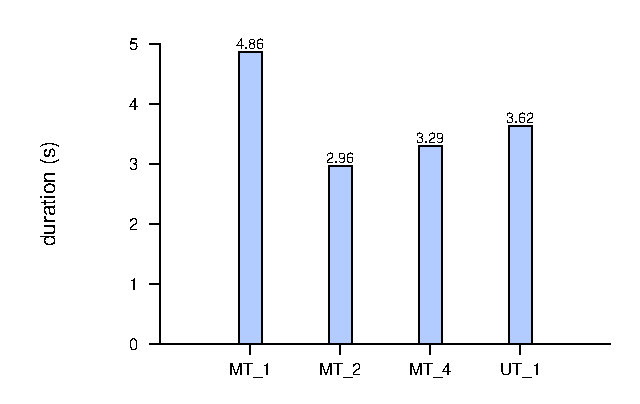
\includegraphics{imgs/tmpfscreate}
\includegraphics{imgs/tmpfscreate2}
\caption[Cost of atomic memory bus locks on a twin core host]{
\textbf{Cost of atomic memory bus locks on a twin core host.}
The first figure presents the raw measurements and the second figure
presents the normalized durations per physical processor.
\textit{MT} means a multiprocessor rump kernel with hardware atomic
locks and \textit{UT} designates a uniprocessor rump kernel without
hardware atomic locks.  The number designates the amount of threads
concurrently executing within the rump kernel.  Notably,
in the case of four threads there are twice as many threads executing
within the rump kernel as there are physical CPUs.
}
\label{fig:tmpfscreate}
\end{figure}
\clearpage

The kernel with uniprocessor locking performs 34\% better than the
multiprocessor version on a uniprocessor rump kernel.  This significant
difference can be explained by the fact that creating files on
memory file systems (\verb+rump_sys_open(O_CREAT)+) is very
much involved with taking and releasing locks (such as file descriptor
locks, directory locks, file object locks ...) and very little
involved with I/O or hypervisor calls.  To verify our results, we
examined the number of mutex locks and reader/writer locks and we
found out they are taken 5,438,997 and 1,393,596 times, respectively.
This measurement implies the spinlock/release cycle fastpath in the 100ns range,
which is what we would expect from a Core2 CPU on which the test was
run.  The MT\_4 case is slower than MT\_2, because the test host has
only two physical cores, and four threads need to compete for the same
physical cores.

The multiprocessor version where the number of threads and virtual
CPUs matches the host CPU allocation wins in wall time.  However,
if it is possible to distribute work in single processor kernels
on all host CPUs, they will win in total performance due to
IPC overhead being smaller than memory bus locking
overhead~\cite{baumann:multikernel}.

\subsection{Application Interfaces to the Rump Kernel}

Application interfaces are used by clients to request services from
the rump kernel.  Having the interfaces provided as part of the
rump kernel framework has two purposes: 1) it provides a C level
prototype for the client 2) it wraps execution around the rump kernel
entry and exit points, \ie thread context management and rump kernel
virtual CPU scheduling.

The set of available interfaces depends on the type of the client.
Since the rump kernel provides a security model for remote clients,
they are restricted to the system call interface --- the system
call interface readily checks the appropriate permissions of a
caller.  A local client and a microkernel server's local client 
are free to call any functions they desire.  We demonstrated the
ability to call arbitrary kernel interfaces
with the example on how to access the BPF driver without going
through the file system (Figure~\ref{fig:bpfdirect}).  In that
example we had to provide our own prototype and execute the entry
point manually, since we did not use predefined application
interfaces.

\subsubsection{System Calls}
\label{sect:syscallentry}

On a regular NetBSD system, a user process calls the kernel through
a stub in libc.  The libc stub's task is to trap into the kernel.
The kernel examines the \textit{trapframe} to see which system call
was requested and proceeds to call the system call handler.  After
the call returns from the kernel, the libc stub sets \texttt{errno}.

We are interested in preserving the standard libc application interface
signature for rump kernel clients.  Preserving the signature will make
using existing code in rump kernel clients easier, since the calling
convention for system calls will remain the same.  In this section we
will examine how to generate handlers for rump kernels with minimal
manual labor.  All of our discussion is written against how system calls
are implemented in NetBSD.  We use \texttt{lseek()} as an example
of the problem and our solution.

The signature of the \verb+lseek()+ system call stub in libc is as
follows:

{\small
\begin{verbatim}
off_t
lseek(int fildes, off_t offset, int whence)
\end{verbatim}}

Prototypes are provided in header files.  The header file
varies from call to call.  For example, the prototype of
\texttt{lseek()} is made available to an application by including
the header file \texttt{<unistd.h>} while \texttt{open()} comes from
\texttt{<fcntl.h>}.  The system call prototypes provided in the
header files are handwritten.  In other words, they are not autogenerated.
On the other hand, almost all libc stubs are autogenerated
from a list of system calls.  There are some manually written
exceptions for calls which do not fit the standard mould, \eg \texttt{fork()}.
Since the caller of the libc stub arranges arguments according to
the platform's calling convention per the supplied prototype and the kernel
picks them up directly from the trapframe, the libc stub in principle
has to only execute the trap instruction to initiate the handling of
the system call.

In contrast to the libc application interface, the signature of
the kernel entry point for the handler of the lseek system call
is:

{\small
\begin{verbatim}
int
sys_lseek(struct lwp *l, const struct sys_lseek_args *uap, register_t *rv)
\end{verbatim}}

This function is called by the kernel trap handler after it has copied
parameters from the trapframe to the args structure.

Native system calls are described by a master file in kernel source
tree located at \texttt{sys/kern/syscalls.master}.  The script
\texttt{sys/kern/makesyscalls.sh} uses the data file to autogenerate,
among other things, the above prototype for the in-kernel implementation
and the definition of the args structure.

\begin{figure}[t]
{\tt \scriptsize  
\begin{verbatim}
off_t
rump___sysimpl_lseek(int fd, off_t offset, int whence)
{
        register_t retval[2] = {0, 0};
        int error = 0;
        off_t rv = -1;
        struct sys_lseek_args callarg;

        SPARG(&callarg, fd) = fd;
        SPARG(&callarg, PAD) = 0;
        SPARG(&callarg, offset) = offset;
        SPARG(&callarg, whence) = whence;

        error = rsys_syscall(SYS_lseek, &callarg, sizeof(callarg), retval);
        rsys_seterrno(error);
        if (error == 0) {
                if (sizeof(off_t) > sizeof(register_t))
                        rv = *(off_t *)retval;
                else
                        rv = *retval;
        }
        return rv;
}
\end{verbatim}}
\caption[Call stub for \texttt{rump\_sys\_lseek()}]{
\textbf{Call stub for \texttt{rump\_sys\_lseek()}.}
The arguments from the client are marshalled into the argument structure
which is supplied to the kernel entry point.  The execution of the system
call is requested using the \texttt{rsys\_syscall()} routine.  This routine
invokes either a direct function call into the rump kernel or a remote request,
depending on if the rump kernel is local or remote, respectively.
}
\label{fig:rumpsyslseek}
\end{figure}

We added support to the makesyscalls script for generating the necessary
wrappers and headers for rump kernel clients.  For a caller to be
able to distinguish between a native system call and a rump kernel
system call, the latter is exported with a \verb+rump_sys+-prefix, \eg
\verb+rump_sys_lseek()+.  The makesyscalls script generates
rump system call prototypes to
\verb+sys/rump/include/rump/rump_syscalls.h+.  A wrapper which
takes care of arranging the function parameters into the args
structure is generated into
\verb+sys/rump/librump/rumpkern/rump_syscalls.c+ --- in our example
this arranging means moving the arguments that \verb+rump_sys_lseek()+ was
called with into the fields of \verb+struct sys_lseek_args+.  The
wrapper for lseek is presented in Figure~\ref{fig:rumpsyslseek}.
The name of the wrapper in the illustration does not match
\verb+rump_sys_lseek()+
but the reference will be correctly translated by an alias
in the rump system call header.  We will not go into details,
except to say that the reason for it is to support compatibility
system calls.  For interested parties, the details are available in
the \verb+rump_syscalls.h+ header file.

The same wrapper works both for local and remote clients.  For a
local client, \verb+rsys_syscall()+ does a function call into the
rump kernel, while for a remote client it invokes a remote procedure
call so as to call the rump kernel.  Remote clients are discussed
in more detail in Section~\ref{sect:sysproxyimpl}.  In both cases,
the implementation behind \verb+rsys_syscall()+ calls the rump
kernel entry and exit routines.

While modifying the makesyscalls script to generate prototypes and
wrappers, we ran into a number of unexpected cases:

\begin{enumerate}
\item   Almost all system calls return -1 (or \texttt{NULL}) in
	case of an error and set the \texttt{errno} variable to
	indicate which error happened.  However, there are exceptions.
	For example, the
	\verb+posix_fadvise()+ call is specified to return an error number
	and not to adjust \texttt{errno}.  In libc
	this discrepancy between error variable
	conventions is handled by a field in the Makefile which
	autogenerates syscall stubs.  For our purposes of
	autogeneration, we added a \texttt{NOERR} flag to
	syscalls.master.  This flag causes the generator to create
	a stub which does not set \texttt{errno}, much like what
	the libc build process does.

\item   Some existing software looks only at \texttt{errno} instead
	of the system call's return value.  Our initial implementation
	set \texttt{errno} only in case the system call returned failure.
	This implementation caused such software to not function properly
	and we adjusted \texttt{errno} to always be set to reflect the
	value from the latest call.

\item   System calls return three values from the kernel:
	an integer and an array containing two register-size values
	(the \verb+register_t *rv+ parameter).  In the typical
	case, the integer carries \texttt{errno} and \texttt{rv[0]}
	carries the return value.  In almost all cases the second
	element of the register vector can be ignored.  The first
	exception to this rule is the system call \texttt{pipe(int
	fildes[2])}, which returns two file descriptors from
	the kernel:  one in \texttt{rv[0]} and the other in
	\texttt{rv[1]}.  We handle \texttt{pipe()} as a special
	case in the generator script.

\item   The second exception to the above is the \texttt{lseek()}
	call on 32bit architectures.  The call returns a 64bit
	\verb+off_t+~\footnote
	{
		\texttt{off\_t} is always 64bit on NetBSD
		instead of depending on the value of
		\texttt{\_FILE\_OFFSET\_BITS} which used on for
		example Linux and Solaris.
	}
	with the low bits occupying one register and the high
	bits the other one.  Since NetBSD supports all combinations
	of 32bit, 64bit, little endian and big endian architectures,
	care had to be taken to have the translation from a
	two-element \verb+register_t+ vector to a variable work
	for all calls on all architectures.  We use a
	compile-time check for data type sizes and typecast
	accordingly.  To see why the check is required, consider
	the following.  If the typecast is never done, lseek breaks on
	32bit architectures.  If the typecast to the return type is
	done for all calls, system calls returning an integer break on
	64bit big-endian architectures.

\begin{figure}[t]
{\tt \scriptsize  
\begin{verbatim}
    [ .... ]
    2194:       e8 fc ff ff ff          call   2195 <rump___sysimpl_lseek+0x52>
    2199:       85 db                   test   %ebx,%ebx
    219b:       75 0c                   jne    21a9 <rump___sysimpl_lseek+0x66>
    219d:       8b 45 f4                mov    0xfffffff4(%ebp),%eax
    21a0:       8b 55 f8                mov    0xfffffff8(%ebp),%edx
    21a3:       83 c4 24                add    $0x24,%esp
    21a6:       5b                      pop    %ebx
    21a7:       5d                      pop    %ebp
    21a8:       c3                      ret    
    [ .... ]
\end{verbatim}}
\caption[Compile-time optimized \texttt{sizeof()} check]{
\textbf{Compile-time optimized \texttt{sizeof()} check.}
The assembly of the generated code compiled for i386 is presented.
}
\label{fig:lseekasm}
\end{figure}

	The above is not the only way to solve the problem.  The
	makesyscalls.sh script detects 64bit return values and
	sets the \verb+SYCALL_RET_64+ flag in a system call's
	description.  We could have hooked into the facility and created
	a special wrapper for lseek without the ``\texttt{if
	(sizeof())}'' clause.  The compiled code is the same for
	both approaches (Figure~\ref{fig:lseekasm}), so the choice
	is a matter of taste instead of runtime performance.

\item   Some calling conventions (\eg ARM~EABI) require
	64bit parameters to be passed in even numbered registers.
	For example, consider the lseek call.  The first parameter
	is an integer and is passed to the system call in register~0.
	The second parameter is 64bit, and according to the ABI
	it needs to be passed in registers~2+3 instead of registers~1+2.
	To ensure the alignment constraint matches in the kernel,
	the system call description table syscalls.master contains
	padding parameters.  For example, lseek is defined as
	\verb+lseek(int fd, int pad, off_t offset, int whence)+.
	Since ``pad'' is not a part of the application API, we
	do not want to include it in the rump kernel system call
	signature.  However, we must include padding in the
	\verb+struct sys_lseek_args+ parameter which is passed to
	the kernel.  We solved the issue by first renaming all pad
	parameters to the uppercase ``PAD'' to decrease the
	possibility of conflict with an actual parameter called
	``pad''.  Then, we modified makesyscalls.sh to ignore all
	parameters named ``PAD'' for the application interface
	side.
\end{enumerate}

A possibility outside of the scope of this work is to examine if
the libc system call stubs and prototypes can now be autogenerated
from \texttt{syscalls.master} instead of requiring separate code
in the NetBSD libc Makefiles and system headers.

\subsubsection{vnode Interface}

The vnode interface is a kernel internal interface.  The vnode
interface routines take a vnode object along with other parameters,
and call the respective method of the file system associated with
the vnode.  For example, the interface for reading is the following:
\verb+int VOP_READ(struct vnode *, struct uio *, int, kauth_cred_t)+;
if the first parameter is a pointer to a FFS vnode, the call will be
passed to the FFS driver.

The rump vnode interface exports the vnode interfaces
to rump kernel clients.  The intended users are microkernel file servers
which use rump kernels as backends.  The benefits for
exporting this interface readily are the ones we listed in the
beginning of this section: a prototype for client code and
automated entry/exit point handling.

\begin{figure}[t]
{\tt \scriptsize  
\begin{verbatim}
int
RUMP_VOP_READ(struct vnode *vp, struct uio *uio, int ioflag, struct kauth_cred *cred)
{
        int error;

        rump_schedule();
        error = VOP_READ(vp, uio, ioflag, cred);
        rump_unschedule();

        return error;
}
\end{verbatim}}
\caption[Implementation of \texttt{RUMP\_VOP\_READ()}]{
\textbf{Implementation of \texttt{RUMP\_VOP\_READ()}.}
The backend kernel call is wrapped around the rump kernel entrypoint
and exitpoint.
}
\label{fig:rumpvopread}
\end{figure}

The wrappers for the vnode interface are simpler than those of the
system call interface.  This simplicity is because there is no need translate
parameters and we can simply pass them on to the kernel internal
interface as such.  To distinguish between the internal implementation
and the rump application interface, we prefix rump client vnode
interfaces with \verb+RUMP_+.

The kernel vnode interface implementations and prototypes are
autogenerated from the file \verb+sys/kern/vnode_if.src+ by
\verb+sys/kern/vnode_if.sh+.
We made the script to generate our prototypes into
\verb+sys/rump/include/rump/rumpvnode_if.h+ and wrapper functions
into \verb+sys/rump/librump/rumpvfs/rumpvnode_if.c+.  An example
result showing the \verb+RUMP_VOP_READ()+ interface is presented in
Figure~\ref{fig:rumpvopread}.  The \verb+VOP_READ()+ routine called
by the wrapper is the standard implementation which is extracted
into a rump kernel from \verb+sys/kern/vnode_if.c+.


\subsubsection{Interfaces Specific to Rump Kernels}

Some interfaces are available only in rump kernels, for example the
lwp/process context management interfaces
(\manpageref{rumplwproc.3}{rump\_lwproc.3}).  In a similar fashion
to other interface classes we have discussed, we supply autogenerated
prototypes and wrappers.

The application interface names are prefixed with \verb+rump_pub_+
(shorthand for public).  The respective internal interfaces are
prefixed \verb+rump_+.  As an example, we present the wrapper for
\verb+rump_pub_lwproc_rfork()+ in Figure~\ref{fig:rumppubrfork}.
The public interface wraps the internal interface around the entrypoint
and exitpoint.

The master files for rump kernel interfaces are contained in the
subdirectory of each faction in an \textit{.ifspec} file.  The
script \texttt{sys/rump/librump/makeifspec.sh} analyzes this
file and autogenerates the prototypes and wrappers.

\begin{figure}[t]
{\tt \scriptsize  
\begin{verbatim}
int
rump_pub_lwproc_rfork(int arg1)
{
        int rv;

        rump_schedule();
        rv = rump_lwproc_rfork(arg1);
        rump_unschedule();

        return rv;
}
\end{verbatim}}
\caption[Application interface implementation of lwproc \texttt{rfork()}]{
\textbf{Application interface implementation of lwproc \texttt{rfork()}.}
The backend kernel call is wrapped around the rump kernel entrypoint
and exitpoint.
}
\label{fig:rumppubrfork}
\end{figure}

Additionally, there exist bootstrap interfaces
which can be called only before the rump kernel is bootstrapped.
An example is \verb+rump_boot_sethowto()+ which sets the
\texttt{boothowto} variable.  Since there is no virtual
CPU to schedule before bootstrap, no entry/exit wrappers are
necessary.  These bootstrap interfaces provided as non-generated prototypes
in \verb+sys/rump/include/rump/rump.h+.


\subsection{Rump Kernel Root File System}
\label{sect:rumpfs}

Full operating systems require a root file system with persistent
storage for files such as \texttt{/bin/ls} and \texttt{/etc/passwd}.
A rump kernel does not inherently require such files.  This relaxed
requirement is because a rump kernel does not have a default userspace
and because client binaries are executed outside of the rump kernel.
However, specific drivers or clients may require file system support for example
to open a device, load firmware or access a file system image.  In some
cases, such as for firmware files and file system images, it is likely
that the backing storage for the data to be accessed resides on the host.

We explicitly want to avoid mandating the association of persistent
storage with a rump kernel because the storage image requires setup
and maintenance and would hinder especially one-time invocations.
It is not impossible to store the file system
hierarchy and data required by a specific rump kernel instance on
persistent storage.  We are merely saying it is not required.

A file system driver called \textit{rumpfs}
was written.  It is implemented in the source module
\verb+sys/rump/librump/rumpvfs/rumpfs.c+.  Like \textit{tmpfs},
rumpfs is an in-memory file system.  Unlike tmpfs, which is as fast
and as complete as possible, rumpfs is as lightweight as possible.
Most rumpfs operations have only simple implementations and support
for advanced features such as rename and NFS export has been omitted.
If these features are desired, an instance of tmpfs can be mounted
within the rump kernel when required.  The lightweight implementation
of rumpfs makes the compiled size 3.5 times smaller than that of
tmpfs.

By convention, file system device nodes are available in \texttt{/dev}.
NetBSD does not feature a device file system which dynamically
creates device nodes based on the drivers in the kernel.
A standard installation of NetBSD relies on precreated
device nodes residing on persistent storage.  We work around this
issue in two ways.  First, during bootstrap, the rump kernel VFS
faction generates a selection of common device nodes such as
\texttt{/dev/zero}.  Second, we added support to various driver
attachments to create device driver nodes when the drivers are
attached.  These adjustments avoid the requirement to have persistent
storage mounted on \texttt{/dev}.

\subsubsection{Extra-Terrestrial File System}
\label{sect:etfs}

The Extra-Terrestrial File System (\textit{etfs}) interface provides
a rump kernel with access to files on the host.  The
etfs (\manpageref{rumpetfs.3}{rump\_etfs.3}) interface is used
to register host file mappings with rumpfs.  Fundamentally, the
purpose of etfs is the same as that of a \textit{hostfs} available
on most full system virtualization solutions.  Unlike a hostfs,
which typically mounts a directory from the host, etfs is oriented
towards mapping individual files.  The interface allows the
registration of type and offset translators for individual host
files; a feature we will look at more closely below.  In addition,
etfs only supports reading and writing files and cannot manipulate
the directory namespace on the host.  This I/O-oriented approach
avoids issues such as how to map permissions on newly created hostfs
files.  Furthermore, it makes etfs usable also on hosts which do not
support a directory namespace.

The mapping capability of etfs is hooked up to the lookup operation
within rumpfs.  Recall, a lookup operation for a pathname will
produce an in-memory file system structure referencing the file
behind that pathname.  If the pathname under lookup consists of a
registered etfs key, the in-memory structure will be tagged so that
further I/O operations, \ie read and write, will be directed to
the backing file on the host.

Due to how etfs is implemented as part of the file system lookup routine,
the mapped filenames is not browseable (\ie readdir).  However, it does
not affect the intended use cases such as access to firmware images,
since the pathnames are hardcoded into the kernel.

In addition to taking a lookup key and the backing file path, the
etfs interface takes an argument controlling how the mapped path
is presented inside the rump kernel.  The following three options
are valid for non-directory host files: regular file, character
device or block device.
The main purpose of the type mapping feature is to be able
to present a regular file on the host as a block device in the rump
kernel.  This mapping addresses an implementation detail in the NetBSD
kernel: the only valid backends for disk file systems are block
devices.

Assuming that the host supports a directory namespace,
it is also possible to map directories.
There are two options: a single-level mapping or the mapping of
the whole directory subtree.  For example, if \verb+/rump_a+ from
the host is directory mapped to \verb+/a+ in the rump kernel, it
is possible to access \verb+/rump_a/b+ from \verb+/a/b+ in both
single-level and subtree mappings.  However, \verb+/rump_a/b/c+ is
visible at \verb+/a/b/c+ only if the directory subtree was mapped.
Directory mappings do not allow the use of the type and offset/size
translations, but allow mappings without having to explicitly add
them for every single file.
The original use case for the directory mapping functionality was
to get the kernel module directory tree from \texttt{/stand} on
the host mapped into the rump kernel namespace so that a rump kernel
could read kernel module binaries from the host.

\subsubsection{External Storage}

Another special feature of rumpfs is the possibility to attach external
storage to regular files.  This external storage is provided in the
form of memory, and is made available via files in a zero-copy fashion.
The intent is to allow rump kernels to provide file content
without having to rely on the presence of any block I/O device.
The content itself can be linked into the data segment of the binary
at the time that the binary is built.
External storage is attached by opening a writable file and calling
\verb+rump_sys_ioctl(fd, RUMP_FCNTL_EXTSTORAGE_ADD, ...)+.
Adding external storage is limited to local clients, as pointers
provided by remote clients are meaningless in this context.


\subsection{Attaching Components}

A rump kernel's initial configuration is defined by the components that
are linked in when the rump kernel is bootstrapped.  At bootstrap time,
the rump kernel needs to detect which components were included in the
initial configuration and attach them.  If drivers are loaded at runtime,
they need to be attached to the rump kernel as well.

In this section we go over how loading and attaching components in
a rump kernel is similar to a regular kernel and how it is different.
The host may support static linking, dynamic linking or both.  We include
both alternatives in the discussion.  There are two methods for attaching
components, called \textit{kernel modules} and \textit{rump components}.
We will discuss both and point out the differences.  We start the
discussion with kernel modules.

\subsubsection{Kernel Modules}
\label{sect:extending}

In NetBSD terminology, a driver which can be loaded and unloaded
at runtime is said to be \textit{modular}.  The loadable binary
image containing the driver is called a \textit{kernel module}, or
\textit{module} for short.  We adopt the terminology for our
discussion.

The infrastructure for supporting modular drivers on NetBSD has
been available since NetBSD~5.0~\footnote
{
	NetBSD~5.0 was released in 2009.  Versions prior to 5.0
	provided kernel modules through a different mechanism called
	Loadable Kernel Modules (\textit{LKM}).  The modules
	available from 5.0 onward are incompatible with the old
	LKM scheme.  The reasons why LKM was retired in favor of
	the new system are available from mailing list archives
	and beyond the scope of this document.
}.
Some drivers offered by NetBSD are modular, and others are being
converted.  A modular driver knows how to attach to the kernel and detach
from the kernel both when it is statically included and when it is loaded
at runtime.  A non-modular driver does not know.

NetBSD divides kernel modules into three classes depending on their
source and when they are loaded.  These classes are summarized in
Table~\ref{tab:kernmod}.  Builtin modules are linked into the kernel
image when the kernel is built.  The bootloader can load kernel modules
into memory at the same time as it loads the kernel image.  These modules
must later be linked by the kernel during the bootstrap process.  Finally,
at runtime modules must be both loaded and linked by the kernel.

\begin{table}[]
\begin{tabular}{|l|l|l|l|}
\hline
source & loading & linking & initiated by \\
\hline
\hline
builtin & external & external & external toolchain \\
\hline
bootloader & external & kernel & bootloader \\
\hline
file system & kernel & kernel & syscall, kernel autoload \\
\hline
\end{tabular}
\caption[Kernel module classification]{
\textbf{Kernel module classification.}
These categories represent the types of kernel modules that were readily
present in NetBSD independent of this work.
}
\label{tab:kernmod}
\end{table}

The fundamental steps of loading a kernel module on NetBSD at
runtime are:

\begin{enumerate}
\item	The kernel module is loaded into the kernel's address space.

\item   The loaded code is linked with the kernel's symbol table.

\item   The module's init routine is run.  This routine informs other kernel
	subsystems that a new module is present.  For example, a
	file system module at a minimum informs the VFS layer that
	it is possible to mount a new type of file system.
\end{enumerate}

After these steps have been performed, code from the newly loaded
kernel module can be used like it had been a part of the original
monolithic kernel build.  Unloading a kernel module is essentially
reversing the steps.

We divide loading a module into a rump kernel in two separate cases
depending on a pivot point in the execution: the bootstrapping of the
rump kernel by calling \verb+rump_init()+.  The officially supported way
of including modules in rump kernels is to have them loaded and linked
(\ie steps 1+2) before \verb+rump_init()+ is called.  This may be done
either by linking them into a static image, or, on hosts where dynamic
linking is supported, loading and linking the component after \verb+main()+
is called but before \verb+rump_init()+ is called.  Modules loaded that
way are essentially builtin modules.

We also point out that on some hosts, especially userspace, it is
possible to load components after \verb+rump_init()+ by using the host
dynamic linker and then calling \verb+rump_pub_module_init()+.  However,
will we not discuss the latter approach in this document.

\subsubsection*{init/fini}

A NetBSD kernel module defines an init routine
(``\verb+modcmd_init+'') and a fini routine (``\verb+modcmd_fini+'')
using the \verb+MODULE()+ macro.  The indicated routines attach
and detach the module with respect to the kernel.  The \verb+MODULE()+
macro creates a structure (\texttt{struct modinfo}) containing that
information.  We need to locate the structure at runtime so that the
init routine can be run to complete module loading step ``3''.  The method
of locating the \texttt{modinfo} structures depends on the platform.
There are two functionally equivalent options, but they have different
platform requirements.

\begin{enumerate}
\item	A pointer to the structure is placed into a \verb+.rodata+ section
	called \texttt{modules}.  At linktime, the linker generates
	\verb+__start_section+ and \verb+__end_section+ symbols.
	At runtime, all present modules can be found by traversing pointers
	in the memory between these two symbols.  Notably, not all linkers
	can be coerced into generating these symbols.
	Furthermore, the scheme is
	not directly compatible with dynamic linkers because a dynamic
	linker cannot produce a global pair of such symbols -- consider
	the scenario where libraries are loaded at runtime.  Therefore,
	if this scheme is to be used with dynamic linking, each shared
	object must be examined separately.

\item	The structure is located via
	\verb+__attribute__((__constructor__))+.  We cannot make any
	assumptions about when the constructor runs, and therefore the
	constructor only places the structure on a linked list.
	This linked list is traversed when the rump kernel boots.
	The constructor is a static function generated by the
	\texttt{MODULE()} macro.  Notably, this scheme requires platform
	support for running constructors.
\end{enumerate}


\subsubsection*{The NetBSD Kernel Linker}

Using the NetBSD kernel linker means loading the module from the
file system after \verb+rump_init()+ and letting the code in
\verb+sys/kern/subr_kobj.c+ handle linking.  This linker is included
as part of the base of a rump kernel.  The in-kernel linker supports
only relocatable objects (with ELF, type \verb+ET_REL+), not shared
libraries.

Since linking is performed in the [rump] kernel, the [rump] kernel
must be aware of the addresses of the symbols it exports.  For
example, for the linker to be able to satisfy an unresolved symbol
to \verb+kmem_alloc()+, it must know where the implementation of
\verb+kmem_alloc()+ is located in that particular instance.  In a
regular kernel the initial symbol table is loaded at bootstrap time
by calling the \verb+ksyms_addsyms_explicit()+ or mostly equivalent
\verb+ksyms_addsyms_elf()+ routine.

In the current rumpuser hypercall revision, the symbol table is populated
by the
\verb+rumpuser_dl_bootstrap()+ hypercall, which is always called during
rump kernel bootstrap.  For the next hypercall revision, the plan is to
make symbol loading a just-in-time operation which is called only if
the in-kernel linker is used.  This change is planned because loading
the symbol table -- and in dynamically linked environments harvesting
it for loading -- is a time-consuming operating.  Based on experience,
the use of the in-kernel linker is a rare operation, and unconditionally
populating the symbol table is therefore wasteful.

The in-kernel linker itself works the same way as in a regular kernel.
Loading a module can be initiated either by a client by using the
\texttt{modctl()} system call.  Notably, the kernel module is loaded
from the rump kernel file system namespace, so only rump kernels with
the file system faction can support the in-kernel linker.


\subsubsection{Modules: Supporting Standard Binaries}
\label{sect:abicompat}

By a binary kernel module we mean a kernel module object file
built for the regular monolithic kernel and shipped with NetBSD in
\verb+/stand/$arch/release/modules+.  Support for binary kernel
modules means these objects can be loaded and linked into a rump
kernel and the drivers used.  This support allows a
rump kernel to use drivers for which source code is not
available.  Short of a full virtual machine (\eg QEMU), rump kernels
are the only form of virtualization in NetBSD capable of using
binary kernel modules without recompilation.

There are two requirements for using binary kernel modules to be possible.
First, the kernel module must not contain any CPU instructions
which cannot be executed in unprivileged mode.  As we examined in
Section~\ref{sect:privinst}, drivers do not contain privileged
instructions.  Second, the rump kernel and the host kernel must share
the same binary interface (ABI).

In practical terms, ABI compatibility means that the rump kernel
code does not provide its own headers to override system headers and therefore
all the data type definitions are the same for a regular kernel
and a rump kernel.  Problematic scenarios arise because, mainly due to historical reasons,
some architecture specific kernel interfaces are provided as macros
or inline functions.  This approach does
not produce a clean interface boundary, as at least part of the
implementation is leaked into the caller.  From our perspective,
this leakage means that providing an alternate interface is more difficult.

Shortly before we started investigating kernel module compatibility,
some x86 CPU family headers were changed from inline/macro definitions
to function interfaces by another NetBSD developer.  The commit message\footnote
{
	revision 1.146 of \texttt{sys/arch/i386/include/cpu.h}
}
states that the change was done to avoid ABI instability issues with
kernel modules.  This change essentially solved our problem with
inlines and macros.  It also
reinforced our belief that the anykernel architecture follows naturally
from properly structured code.

A remaining example of macro use in an interface is the \textit{pmap}
interface.  The pmap is the interface to the architecture dependent
memory management features.  The interface specification explicitly
allows some parts of the interface to be implemented as macros.
Figure~\ref{fig:pmapmacros} illustrates how the x86 pmap header
overrides the MI function interface for \verb+pmap_is_modified()+.
To be x86 kernel ABI compatible we provide an implementation
for \verb+pmap_test_attrs()+ in the rump kernel base
(\verb+sys/rump/librump/rumpkern/arch/i386/pmap_x86.c+).

\begin{figure}[t]
\begin{flushleft}
sys/arch/x86/include/pmap.h:
{\tt \scriptsize  
\begin{verbatim}
#define pmap_is_modified(pg)            pmap_test_attrs(pg, PG_M)
\end{verbatim}}

sys/uvm/uvm\_pmap.h (MI definition):
{\tt \scriptsize  
\begin{verbatim}
#if !defined(pmap_is_modified)
bool            pmap_is_modified(struct vm_page *);
#endif
\end{verbatim}}
\end{flushleft}
\caption[Comparison of \texttt{pmap\_is\_modified} definitions]{
\textbf{Comparison of \texttt{pmap\_is\_modified} definitions.}
The definition specific to the \textit{i386} port causes a dereference of the
symbol \texttt{pmap\_test\_attrs()}, while for all ports which do not
override the definition, \texttt{pmap\_is\_modified()} is used.
}
\label{fig:pmapmacros}
\end{figure}

Due to the MD work required, the kernel module ABI support is
currently restricted to the AMD64 and i386 architectures.  Support
for AMD64 has an additional restriction which derives from the
addressing model used by kernel code on AMD64.  Since most AMD64
instructions accept only 32bit immediate operands, and since an OS
kernel is a relatively small piece of software, kernel code is
compiled with a memory model which assumes that all symbols are
within the reach of a 32bit offset.  Since immediate operands are
sign extended, the values are correct when the kernel is loaded in
the upper 2GB of AMD64's 64bit address space~\cite{amd64abi}.  This
address range is not available to user processes at least on NetBSD.
Instead, we used the lowest 2GB --- the lowest 2GB is the same as
the highest 2GB without sign-extension.  As long as the rump kernel
and the binary kernel module are loaded into the low 2GB, the binary
kernel module can be used as part of the rump kernel.

\begin{figure}[t]
\begin{flushleft}
sys/arch/x86/include/cpu.h:
{\tt \scriptsize  
\begin{verbatim}
#define curlwp                  x86_curlwp()
\end{verbatim}}

sys/arch/sparc64/include/\{cpu,param\}.h (simplified for presentation):
{\tt \scriptsize  
\begin{verbatim}
#define curlwp          curcpu()->ci_curlwp
#define curcpu()        (((struct cpu_info *)CPUINFO_VA)->ci_self)
#define CPUINFO_VA      (KERNEND+0x018000)
#define KERNEND         0x0e0000000     /* end of kernel virtual space */
\end{verbatim}}
\end{flushleft}
\caption[Comparison of \texttt{curlwp} definitions]{
\textbf{Comparison of \texttt{curlwp} definitions.}
The \textit{i386} port definition results in a function symbol
dereference, while the \textit{sparc64} port definition causes a
dereference to an absolute memory address.
}
\label{fig:curlwp}
\end{figure}

For architectures which do not support the standard kernel
ABI, we provide override machine headers under the directory
\texttt{sys/rump/include/machine}.  This directory is specified first
in the include search path for rump kernel compilation, and therefore
headers contained in there override the NetBSD MD headers.  Therefore,
definitions contained in the headers for that directory override the
standard NetBSD definitions.  This way we can override problematic
definitions in machine dependent code.  An example of what we consider
problematic is SPARC64's definition of \texttt{curlwp}, which we
previously illustrated in Figure~\ref{fig:curlwp}.  This approach
allows us to support rump kernels on all NetBSD architectures without
having to write machine specific counterparts or edit the existing MD
interface definitions.  The only negative impact is that architectures
which depend on override headers cannot use binary kernel modules and
must operate with the components compiled specifically for rump kernels.

Lastly, the kernel module must be converted to the rump kernel
symbol namespace (Section~\ref{chap:rumpns}) before linking.  This
conversion can be done with the \texttt{objcopy} tool similar to what is done
when components are built.  However, using \texttt{objcopy} would require generating
another copy of the same module file.  Instead of the objcopy
approach, we modified the module load path in
\verb+sys/kern/subr_kobj.c+ to contain a call to \verb+kobj_renamespace()+
after the module has been read from storage but before it is linked.
On a regular kernel this interface is implemented by a null operation,
while in a rump kernel the call is implemented by a symbol renaming
routine in \verb+sys/rump/librump/rumpkern/kobj_rename.c+.  Since
the translation is done in memory, duplicate files are not required.
Also, it enables us to autoload binary modules directly from the host, as
we describe next.

\subsubsection{Rump Component Init Routines}

In the previous section we discussed the attachment of drivers that
followed the kernel module framework.  Now we discuss the runtime
attachment of drivers that have not yet been converted to a kernel
module, or code that applies to a only rump kernel environment.

If a driver is modular, the module's init routine should be preferred
over any rump kernel specific routines since the module framework is more generic.
However, a module's init routine is not always enough for a rump
kernel.  Consider the following cases.  On a regular system, parts of
the kernel are configured by userspace utilities.  For example,
the Internet address of the loopback interface (\texttt{127.0.0.1}) is configured by the
\textit{rc scripts} instead of by the kernel.  Another example is the creation
of device nodes on the file system under the directory \texttt{/dev}.  NetBSD does
not have a dynamic device file system and device nodes are pre-created
with the \texttt{MAKEDEV} script.  Since a rump kernel does not
have an associated userland or a persistent root file system, these
configuration actions must be performed by the rump kernel itself.
A rump component init routine may be created to augment the
module init routine.

By convention, we place the rump component init routines in the
component's source directory in a file called \verb+$name_component.c+,
\eg \verb+bpf_component.c+.
To define an init routine,  the component should use the
\verb+RUMP_COMPONENT()+ macro.  The use of this macro serves the
same purpose as the \verb+MODULE()+ macro and ensures that the init
routine is automatically called during rump kernel bootstrap.

The \verb+RUMP_COMPONENT()+ macro takes as arguments a single
parameter indicating when the component should be initialized
with respect to other components.
This specifier is required because of interdependencies of components
that the NetBSD kernel code imposes.  For example, the networking
domains must be attached before interfaces can be configured.  It
is legal (and sometimes necessary) for components to define several init
routines with different configuration times.
The init level parameters are listed in
Table~\ref{tab:compinit} in order of runtime initialization.  Notably, the
multitude of networking-related initialization levels conveys the
current status of the NetBSD TCP/IP stack: it is not yet modular --- a
modular TCP/IP stack would encode the cross-dependencies in the
drivers themselves.

\begin{table}[]
\begin{tabular}{|l|p{8cm}|}
\hline
level & purpose \\
\hline
\hline
\verb+RUMP_COMPONENT_KERN+ & base initialization which is done before
	any factions are attached \\
\hline
\verb+RUMP_COMPONENT_VFS+ & VFS components \\
\hline
\verb+RUMP_COMPONENT_NET+ & basic networking, attaching of networking domains \\
\hline
\verb+RUMP_COMPONENT_NET_ROUTE+ & routing, can be done only after all
	domains have attached \\
\hline
\verb+RUMP_COMPONENT_NET_IF+ & interface creation (e.g. \texttt{lo0}) \\
\hline
\verb+RUMP_COMPONENT_NET_IFCFG+ & interface configuration, must be done after
	interfaces are created \\
\hline
\verb+RUMP_COMPONENT_DEV+ & device components \\
\hline
\verb+RUMP_COMPONENT_DEV_AFTERMAINBUS+ & device components run which after
	the device tree root (\textit{mainbus}) has attached \\
\hline
\verb+RUMP_COMPONENT_KERN_VFS+ & base initialization which is done
	after the VFS faction has attached, e.g. base components which
	do VFS operations \\
\hline
\verb+RUMP_COMPONENT_SYSCALL+ & establish \textit{non-modular} syscalls
	which are available in the factions present \\
\hline
\verb+RUMP_COMPONENT_POSTINIT+ & misc. components that attach right before
	\verb+rump_init()+ returns \\
\hline
\end{tabular}
\caption[Component classes]{
\textbf{Component classes}.
The \texttt{RUMP\_COMPONENT} facility allows to specify component
initialization at rump kernel bootstrap time.  Due to interdependencies
between subsystems, the component type specifies the order in which
components are initialized.  The order of component initialization is from top
to bottom.  The initializers designated \texttt{DEV}, \texttt{NET}
and \texttt{VFS} are run only if the respective faction is present.
}
\label{tab:compinit}
\end{table}

An example of a component file is presented in
Figure~\ref{fig:component.c}.  The two routines specified in the
component file will be automatically executed at the appropriate
times during rump kernel bootstrap so as to ensure that any
dependent components have been initialized before.  The full source
code for the file can be found from the source tree path
\verb+sys/rump/net/lib/libnetinet/netinet_component.c+.  The
userspace rc~script \texttt{etc/rc/network} provides the equivalent
functionality in a regular monolithic NetBSD setup.

\begin{figure}[]
{\tt \scriptsize  
\begin{verbatim}
RUMP_COMPONENT(RUMP_COMPONENT_NET)
{
        DOMAINADD(inetdomain);

        [ omitted: attach other domains ]
}

RUMP_COMPONENT(RUMP_COMPONENT_NET_IFCFG)
{
        [ omitted: local variables ]

        if ((error = socreate(AF_INET, &so, SOCK_DGRAM, 0, curlwp, NULL)) != 0)
                panic("lo0 config: cannot create socket");

        /* configure 127.0.0.1 for lo0 */
        memset(&ia, 0, sizeof(ia));
        strcpy(ia.ifra_name, "lo0");
        sin = (struct sockaddr_in *)&ia.ifra_addr;
        sin->sin_family = AF_INET;
        sin->sin_len = sizeof(struct sockaddr_in);
        sin->sin_addr.s_addr = inet_addr("127.0.0.1");

        [ omitted: define lo0 netmask and broadcast address ]

        in_control(so, SIOCAIFADDR, &ia, lo0ifp, curlwp);
        soclose(so);
}
\end{verbatim}}
\caption[Example: selected contents of \texttt{netinet\_component.c}]{
\textbf{Example: selected contents of \texttt{netinet\_component.c}.}
The inet domain is attached in one constructor.
The presence of the domain is required for configuring an inet address
for \texttt{lo0}.  The interface itself is provided and created by the
\textit{net} component (not shown).
}
\label{fig:component.c}
\end{figure}


\subsection{I/O Backends}
\label{sect:iobackend}

I/O backends allow a rump kernel to access I/O resources on the host
and beyond.  Access to I/O devices always stems from hypercalls,
and like we learned in Section~\ref{sect:hypercall}, hypercalls for
accessing I/O devices are specific to the bus or device.  For
example, accessing a PCI NIC is completely different from accessing
\texttt{/dev/tap}.

In this section we will discuss the implementation possibilities and
choices for the I/O backends for networking and file systems (block
devices) in userspace.  Other related sections are the ones which
discuss USB via \textit{ugen} (Section~\ref{sect:usb}) and PCI on the
Rumprun unikernel (Section~\ref{sect:pci}).  There is also support
for accessing PCI devices from userspace available at
\url{http://repo.rumpkernel.org/pci-userspace}, but we do not discuss
that implementation in this book.


\subsubsection{Networking}
\label{sect:networking}

The canonical way an operating system accesses the network is via an
interface driver.
The driver is at bottom of the network stack and
has the capability for sending and receiving raw networking
packets.  On most general purpose OSs, sending and receiving raw
network data is regarded as a privileged operation.
Rather, unprivileged programs have only the capability
to send and receive data via the sockets interfaces instead of deciding
the full contents of a networking packet.

\begin{figure}[t]
\includegraphics[width=\linewidth]{imgs/ifcomp}
\caption[Networking options for rump kernels]{
\textbf{Networking options for rump kernels.}
The \textit{virtif}
facility provides a full networking stack by interfacing with, for example, the host's
\textit{tap} driver (depicted).  The \textit{shmem} facility uses interprocess
shared memory to provide an Ethernet-like bus to communicate between
multiple rump kernels on a single host without requiring elevated
privileges on the host.
The \textit{sockin} facility provides unprivileged network access for
all in-kernel socket users via the host's sockets.
}
\label{fig:netcomp}
\end{figure}

We have three distinct cases we wish to support in rump kernels.
The cases are illustrated in Figure~\ref{fig:netcomp} and discussed
next.

\begin{enumerate}
\item   \textbf{full network stack with raw access to the host's
	network}.  In this case the rump kernel can send and receive
	raw network packets.  An example of when this type of access
	is desired is an IP router.  Elevated privileges are
	required, as well as selecting a host device through which
	the network is accessed.

\item   \textbf{full network stack without access to the host's
	network}.  In this use case we are interested in being able
	to send raw networking packets between rump kernels, but
	are not interested in being able to access the network on
	the host.  Automated kernel driver testing in userspace is the main use case for this
	type of setup.  We can fully use all of the networking
	stack layers, with the exception of the physical device
	driver, on a fully unprivileged account without any prior
	host resource allocation.

\item   \textbf{unprivileged use of host's network for sending and
	receiving data}.  In this case we are interested in the
	ability to send and receive data via the host's network,
	but do not care about the IP address associated with our
	rump kernel.  Though sending data via the host's network
	stack requires that the host has a properly configured
	network stack, we argue that this assumption is commonly true.

	An example use case is the NFS client driver:
	we wish to isolate and virtualize the handling of the NFS
	protocol (\ie the file system portion).  However, we still
	need to transmit the data to the server.  Using a full
	networking stack would not only require privileges, but
	also require configuring the networking stack (IP address,
	etc.).  Using the host's stack to send and receive data
	avoids these complications.

	This option is directed at client side services, since all
	rump kernel instances will share the host's port namespace,
	and therefore it is not possible to start multiple instances
	of the same service.
\end{enumerate}

\subsubsection*{Raw network access}

The commonly available way for accessing an Ethernet network from a virtualized
TCP/IP stack running in userspace is to use the \textit{tap} driver
with the \texttt{/dev/tap} device node.  The tap driver presents a file type
interface to packet networking, and raw Ethernet frames can be
received and sent from an open device node using the \texttt{read()} and
\texttt{write()} calls.  If the tap interface on the host is bridged with
a hardware Ethernet interface, access to a physical network is available
since the hardware interface's traffic will be available via the tap
interface as well.  This tap/bridge scenario was illustrated in
Figure~\ref{fig:netcomp}.

The commands for bridging a tap interface on NetBSD are
provided in Figure~\ref{fig:tapbridgecmds}.  Note that IP addresses
are not configured for the tap interface on the host.

\begin{figure}[t]
{\tt \scriptsize
\begin{verbatim}
# ifconfig tap0 create
# ifconfig tap0 up
# ifconfig bridge0 create
# brconfig bridge0 add tap0 add re0
# brconfig bridge0 up
\end{verbatim}
}
\caption[Bridging a tap interface to the host's \texttt{re0}]{
\textbf{Bridging a tap interface to the host's \texttt{re0}.}
The allows the tap device to send and receive network packets via \texttt{re0}.
}
\label{fig:tapbridgecmds}
\end{figure}

The \textit{virt} (\manpageref{virt.4}{virt.4}) network interface driver
we implemented uses hypercalls to open the tap device on the
host and to transmit packets via it.  The source code for the driver is
located in \verb+sys/rump/net/lib/libvirtif+.

Notably, while the tap method is near-ubiquitous and virtualizes
the underlying network device for multiple consumers, it is not
a high-performance option.  At \url{http://repo.rumpkernel.org/}
we host high-performance network driver implementations for DPDK and
netmap~\cite{rizzo:netmap} backends.  While we will not discuss those
implementations in this book, we want to note that the rump kernel side
of the driver is shared between the one use for tap (\ie \textit{virt}).
The difference comes from alternative hypercall implementations.


\subsubsection*{Full network stack without host network access}

Essentially, we need an unprivileged Ethernet-like bus.  All interfaces
which are attached to the same bus will be able to talk to each other
directly, while nodes with interfaces on other buses may be reached via routers.

One option for implementing packet distribution is to use a
userland daemon which listens on a local domain socket~\cite{dike:uml}.
The client kernels use hypercalls to access the local domain socket
of the daemon.  The daemon takes care of passing Ethernet frames to
the appropriate listeners.  The downside of the daemon is that there
is an extra program to install, start and stop.  Extra management is
in conflict with the goals of rump kernels, and that is why we chose
another implementation strategy.

We use shared memory provided by a memory mapped file as the network bus.
The filename is the bus handle --- all network interfaces
on the same bus use the same filename.  The \textit{shmif} driver
(\manpageref{shmif.4}{shmif.4}) in the rump kernel accesses the bus.
Each driver instance accesses one bus, so it is possible to connect a
rump kernel to multiple different busses by configuring multiple drivers.
Since all nodes have full access to bus contents, the
approach does not protect against malicious nodes.  As our main use case
is testing, this lack of protection is not an issue.  Also, the creation of a file on the
host is not an issue, since testing is commonly carried out in a working
directory which is removed after a test case has finished executing.

The shmif driver memory maps the file and uses it as a ring buffer.  The
header contains pointers to the first and last packet and a generation
number, along with bus locking information.  The bus lock is a
spinlock based on cross-process shared memory.  A downside to this
approach is that if a rump kernel crashes while holding the bus
lock, the whole bus will halt.  Since the main purpose of \textit{shmif}
is testing, we do not consider the bus halting a serious flaw.

Sending a packet requires locking the bus and copying the contents of
the packet to the buffer. Receiving requires knowing when to check for
new packets.  It is the job of a hypercall to monitor the bus and wake
up the receive side when the bus changes.  This monitoring is,
for example, implemented by using the \textit{kqueue} facility on BSD
and \textit{inotify} on Linux.  The receive side of the driver
locks the bus and analyzes the bus header.  If there are new packets
for the interface on question, the driver passes them up to the IP layer.

An additional benefit of using a file is that there is always one
ringbuffer's worth of traffic available in a postmortem situation.
The \verb+shmif_dumpbus+ tool
(\manpageref{shmifdumpbus.1}{shmif\_dumpbus.1}) can be used to
convert a busfile into the \textit{pcap} format which the
\texttt{tcpdump} tool understands.  This conversion allows running
a post-mortem tcpdump on a rump kernel's network packet trace.

\subsubsection*{Unprivileged use of the host's network in userspace}

Some POSIX-hosted virtualization solutions such as QEMU and UML provide
unprivileged zero-configuration network access via a facility called
Slirp~\cite{slirp}.  Slirp is a program which was popular during the
dial-up era.  It enables running a SLIP~\cite{slip} endpoint on top of
a regular UNIX shell without a dedicated IP.  Slirp works by mapping the
SLIP protocol to socket API calls.  For example, when an application on
the client side makes a connection, Slirp processes the SLIP frame from
the client and notices a TCP SYN is being sent.  Slirp then opens a socket
and initiates a TCP connection on it.  Note that both creating a socket
and opening the connection are performed at this stage.  This bundling
happens because opening the socket in the application does not
cause network traffic to be sent, and therefore Slirp is unaware of it.

Since the host side relies only on the socket API, there is no need
to perform network setup on the host.  Furthermore, elevated
privileges are not required for the use of TCP and UDP (except for
opening ports <1024).  On the
other hand, ICMP is not available since using it requires access
to raw sockets on the host.  Also, any IP address configured on
the guest will be purely fictional, since socket traffic sent from
Slirp will use the IP address of the host Slirp is running on.

Since Slirp acts as the peer for the guest's TCP/IP stack, it
requires a complete TCP/IP stack implementation.
The code required for complete TCP/IP processing is sizeable: over 10,000 lines of code.

Also, extra processing power is required, since the traffic needs
to be converted multiple times: the guest converts the application
data to IP datagrams, Slirp converts it back into data and socket
family system call parameters, and the host's TCP/IP stack converts
input from Slirp again to IP datagrams.

\begin{figure}[]
{\tt \scriptsize
\begin{verbatim}
DOMAIN_DEFINE(sockindomain);

const struct protosw sockinsw[] = {
{
    .pr_type = SOCK_DGRAM, /* UDP */
    .pr_domain = &sockindomain,
    .pr_protocol = IPPROTO_UDP,
    .pr_flags = PR_ATOMIC | PR_ADDR,
    .pr_usrreq = sockin_usrreq,
    .pr_ctloutput = sockin_ctloutput,
},{
    .pr_type = SOCK_STREAM, /* TCP */
    .pr_domain = &sockindomain,
    .pr_protocol = IPPROTO_TCP,
    .pr_flags = PR_CONNREQUIRED | PR_WANTRCVD | PR_LISTEN | PR_ABRTACPTDIS,
    .pr_usrreq = sockin_usrreq,
    .pr_ctloutput = sockin_ctloutput,
}};

struct domain sockindomain = {
    .dom_family = PF_INET,
    .dom_name = "socket_inet",
    .dom_init = sockin_init,
    .dom_externalize = NULL,
    .dom_dispose = NULL,
    .dom_protosw = sockinsw,
    .dom_protoswNPROTOSW = &sockinsw[__arraycount(sockinsw)],
    .dom_rtattach = rn_inithead,
    .dom_rtoffset = 32,
    .dom_maxrtkey = sizeof(struct sockaddr_in),
    .dom_ifattach = NULL,
    .dom_ifdetach = NULL,
    .dom_ifqueues = { NULL },
    .dom_link = { NULL },
    .dom_mowner = MOWNER_INIT("",""),
    .dom_rtcache = { NULL },
    .dom_sockaddr_cmp = NULL
};
\end{verbatim}}
\caption[sockin attachment]{
\textbf{\textit{sockin} attachment.}
Networking domains in NetBSD are attached by specifying a \texttt{struct
domain}.  Notably, the sockin family attaches a \texttt{PF\_INET}
type family since it aims to provide an alternative implementation for
inet sockets.
}
\label{fig:sockin}
\end{figure}

Our implementation is different from the one described above.  Instead of doing
transport and network layer processing in the rump kernel, we observe
that regardless of what the guest does, processing will be done by the
host.  At best, we would need to undo what the guest did so that we
can feed the payload data to the host's sockets interface.  Instead of
using the TCP/IP protocol suite in the rump kernel, we redefine the
inet domain, and attach our implementation at the \textit{protocol
switch} layer~\cite{stevens:tcpip2}.  We call this new implementation
\textit{sockin} to reflect it being \textbf{sock}et \textbf{in}et.
The attachment to the kernel is illustrated in
Figure~\ref{fig:sockin}.  Attaching at the domain level means
communication from the kernel's socket layer is done with
\textit{usrreq}'s, which in turn map to the host socket API in a very
straightforward manner.  For example, for \verb+PRU_ATTACH+ we call
\texttt{socket()}, for \verb+PRU_BIND+ we call \texttt{bind()}, for
\verb+PRU_CONNECT+ we call \texttt{connect()}, and so forth.  The
whole implementation is 500 lines of code (including whitespace and
comments), making it 1/20th of the size of Slirp.

Since sockin attaches as the Internet domain, it is mutually exclusive
with the regular TCP/IP protocol suite.  Furthermore, since the
interface layer is excluded, the sockin approach is not suitable for
scenarios which require full TCP/IP processing within the virtual
kernel, \eg debugging the TCP/IP stack.  In such cases one of the
other two networking models should be used.  This choice may
be made individually for each rump kernel instance.

\subsubsection{Disk Driver}
\label{chap:diskdriver}

A disk block device driver provides storage medium access and is
instrumental to the operation of disk-based file systems.  The main
interface is simple: a request instructs the driver to read or
write a given number of sectors at a given offset.  The disk driver
queues the request and returns.  The request is handled in an order
according to a set policy, \eg the disk head elevator.  Once the request
is complete, the driver signals the kernel that the request has been
completed.  In case the caller waits for the request to complete, the
request is said to be synchronous, otherwise asynchronous.

There are two ways to provide a disk backend: buffered and unbuffered.
A buffered backend stores writes to a buffer and flushes them to
the backing storage later.  Notably, to maintain file system on-disk
correctness, synchronous writes must still be flushed to storage immediately.
An unbuffered backend will always write to storage immediately.  Examples of
these backend types are a regular file and a character special device,
respectively.

There are three approaches to implementing the block driver
hypercalls using standard userspace interfaces.

\begin{itemize}
\item   \textbf{Use \texttt{read()} and \texttt{write()}
	in caller context}: this is the simplest method.  However,
	this method effectively makes all requests synchronous.
	Additionally, this method blocks other read
	operations when read-ahead is being performed.

\item   \textbf{Asynchronous read/write}: in this model the request is
        handed off to an I/O thread.  When the request has been
        completed, the I/O thread signals completion.

        A buffered backend must flush synchronously executed
        writes.  The only standard interface available for flushing
        is \texttt{fsync()}.  However, it will flush all buffered
        data before returning, including previous asynchronous
        writes.  Non-standard ranged interfaces such as
        \verb+fsync_range()+ exist, but they usually flush at least
        some file metadata in addition the actual data causing
        extra unnecessary I/O.

        A userlevel write to an unbuffered backend goes directly
        to storage.  The system call will return only after the
        write has been completed.  No flushing is required, but
        since userlevel I/O is serialized on Unix, it is not possible
        to issue another write before the first one finishes.  This
        ordering means that a synchronous write must block and wait until
        any earlier write calls have been fully executed.

        The \verb+O_DIRECT+ file descriptor flag causes a write on
        a buffered backend to bypass cache and go directly to
        storage.  The use of the flag also invalidates the cache
        for the written range, so it is safe to use in conjunction
	with buffered I/O.  However, the flag is advisory.  If
	conditions are not met, the I/O will silently fall back to
	the buffer.  The direct I/O method can therefore be used only
	when it is certain that direct I/O applies.

\item   \textbf{Memory-mapped I/O}: this method
        works only for regular files.  The benefits are that the
        medium access fastpath does not involve any system calls
        and that the \texttt{msync()} system call can be portably
        used to flush ranges instead of the whole memory cache.

	The file can be mapped using windows.  Windows provide two
	advantages.  First, files larger than the available VAS
	can be accessed.  Second, in case of a crash, the core dump is only
	increased by the size of the windows instead of the size of the
	entire file.  We found that the number of windows does not have a
	significant performance impact; we default to 16 1MB windows
	with LRU recycling.

        The downside of the memory mapping approach is that to
        overwrite data, the contents must first be paged in, then
        modified, and only after that written.  The pagein step is to
        be contrasted to explicit I/O requests, where it is possible to
        decide if a whole page is being written, and if so, skip pagein
        before write.
\end{itemize}

Of the above, we found that on buffered backends \verb+O_DIRECT+
works best.  Ranged syncing and memory mapped I/O have roughly
equal performance and full syncing performs poorly.


\subsection{Hardware Devices: A Case of USB}
\label{sect:usb}

A general purpose OS kernel USB driver stack may choose to export USB
device access to userspace via the USB generic driver, or \textit{ugen}.
After ugen attaches to a USB bus node, it provides access to the
attached hardware (\ie not the entire USB bus) from userspace via
the \texttt{/dev/ugen<n>} device nodes and read/write/ioctl calls.
Providing access via a device node
means that any entity on the host with the appropriate privileges to
access the device node may communicate with the hardware without having
full access to the device registers.  A key point is that the USB protocol
offered by ugen is essentially unchanged from the USB hardware protocol.
This protocol compatibility allows preexisting kernel drivers to use
ugen without protocol translation.

At the root of the USB bus topology is a \textit{USB host controller}.
It controls all traffic on the USB bus.  All device access on the bus
is done through the host controller using an interface called USBDI, or
USB Driver Interface.  The role of the host controller, along with ugen,
is a detail which makes USB especially suitable for userspace drivers:
we need to implement a host controller which maps USBDI to the ugen
device node instead of having to care about all bus details.

We implemented a host controller called \textit{ugenhc}.  When
the kernel's device autoconfiguration subsystem calls the \textit{ugenhc}
driver to probe the device, the \textit{ugenhc} driver tries to open
\texttt{/dev/ugen} on the host.  If the open is successful, the
host kernel has attached a device to the respective ugen instance
and \textit{ugenhc} can return a successful match.  Next, the \textit{ugenhc}
driver is attached in the rump kernel, along with a USB bus and a
USB root hub.  The root hub driver explores the bus to see which
devices are connected to it, causing the probes to be delivered
first to \textit{ugenhc} and through \texttt{/dev/ugen} to the host
kernel and finally to the actual hardware.  The device driver instance can
be used from the rump kernel just like any other device driver, \eg
USB network interfaces can be used by the networking stack to shuffle
packets.

\subsubsection{Conclusions of the USB Approach}

The USB approach is not recommended for hooking device drivers to rump
kernels.  To implement \textit{ugenhc}, support for the USB protocol
stack must already exist on the host.  Even though USB is supported
by many hosts, the current implementation of \textit{ugenhc} is still
NetBSD-specific.  Furthermore, we found that though in theory access
through \texttt{/dev/ugen} is safe, during development we were able to
tickle the host's USB protocol stack in surprising ways causing host
kernel panics.  Supposedly, this instability is caused by the compound
effect of both the USB protocol stack implementation being huge, and
accessing it via \texttt{/dev/ugen} not being the frequently exercised
access path.


\subsection{Microkernel Servers: Case Study with File Servers}
\label{sect:libp2k}

In this section we investigate using rump kernels as microkernel
style servers for file systems.  Our key motivation is to
prevent a malfunctioning file system driver from damaging the host
kernel by isolating it in a userspace server.

The NetBSD framework for implementing file servers in userspace is
called \textit{puffs}~\cite{kantee:puffs}.  We use puffs to attach
the rump kernel file server to the host's file system namespace.  Conceptually,
after the file system has been mounted, the service works as
follows: a file system request is transported from the host kernel
to the userspace server using puffs.  The server makes a local call
into the rump kernel to
service the request.  When servicing the request is complete, the response is returned
to the host kernel using puffs.  The architecture of this solution
is presented in Figure~\ref{fig:fsserv}.  It is worth noting that
a userlevel application is not the only possible
consumer.  Any VFS user, such as an NFS server running in the host kernel,
is a valid consumer in this model.

\begin{figure}[t]
\includegraphics[height=6cm]{imgs/puffsarch}
\caption[File system server]{
\textbf{File system server.}
The request from the microkernel client is transported by the host kernel
to the rump kernel running providing the kernel file system driver.
Although only system calls are illustrated, page faults created by
the client may be handled by the server as well.
}
\label{fig:fsserv}
\end{figure}


\subsubsection{Mount Utilities and File Servers}

Before a file system can be accessed, it must be mounted.  Standard
kernel file systems are mounted with utilities such as \verb+mount_efs+,
\verb+mount_tmpfs+, etc.  These utilities parse the command line
arguments and call the \texttt{mount()} system call with a file system
specific argument structure built from the command line arguments.  One typical
way of invoking these utilities is to use the \texttt{mount} command
with an argument specifying the file system.  For example,
\verb+mount -t efs /dev/sd0e /mnt+ invokes \verb+mount_efs+ to do
the actual mounting.

Instead of directly calling \texttt{mount()}, our server does the
following: we bootstrap a rump
kernel, mount the file system in the rump kernel, and attach this
process as a puffs server to the host.  All of these tasks are
performed by our mount commands counterparts: \verb+rump_efs+,
\verb+rump_tmpfs+, etc.  The usage of the rump kernel variants is
unchanged from the originals, only the name is different.
To maximize integration, these file~servers share the same command
line argument parsing code with the regular mount utilities.  Sharing
was accomplished by restructuring the mount utilities to provide an interface
for command line argument parsing and by calling those interfaces from
the \verb+rump_xfs+ utilities.

Sharing argument parsing means that the file~servers have the
same syntax.  This feature makes usage interchangeable just by altering the
command name.  We also added a \texttt{rump} option to the
\texttt{mount} command.  For example,
consider the following command: \verb+mount -t efs -o rump /dev/sd0e /mnt+.
It will invoke \verb+rump_efs+ instead of \verb+mount_efs+
and therefore the file system will be mounted with a rump kernel
file system driver.
The \texttt{rump} option works also in
\texttt{/etc/fstab}, as is illustrated in Figure~\ref{fig:orump}.
The flag allows the use of rump kernel file servers to handle specific
mounts such as USB devices and CD/DVD by adding just one option.
The figure also demonstrates how the NFS client (same applies to SMBFS/CIFS)
running inside a rump kernel or the host kernel are completely
interchangeable since the rump kernel drivers use the sockin
networking facility (Section~\ref{sect:networking}) and therefore
share the same IP address with the host.

\begin{figure}[t]
\begin{flushleft}
in-kernel mount:
{\tt \small
\begin{verbatim}
/dev/sd0e               /m/usb          msdos           rw,-u=1000
10.181.181.181:/m/dm    /m/dm           nfs             rw,-p
\end{verbatim}}

equivalent rump kernel file server mount:
{\tt \small
\begin{verbatim}
/dev/sd0e               /m/usb          msdos           rw,-u=1000,rump
10.181.181.181:/m/dm    /m/dm           nfs             rw,-p,rump
\end{verbatim}}
\end{flushleft}
\caption[Use of \texttt{-o rump} in \texttt{/etc/fstab}]{
\textbf{Use of \texttt{-o rump} in \texttt{/etc/fstab}.}
The syntax for a file system served by an in-kernel driver or a rump
kernel is the same apart from the \textit{rump} flag.
}
\label{fig:orump}
\end{figure}

The list of kernel file system drivers available as rump servers
is available in the ``SEE ALSO'' section of the \texttt{mount(8)}
manual page on a NetBSD system.  Support in 5.99.48 consists of ten
disk-based and two network-based file systems.

\subsubsection{Requests: The p2k Library}

We attach to the host as a puffs file server, so the file system
requests we receive are in the format specified by puffs.  We must
feed the requests to the rump kernel to access the backend file
system.  To be able to do so, we must convert the requests to a
suitable format.  Since the interface offered by puffs is close to
the kernel's VFS/vnode~interface~\cite{daemonbook} we can access
the rump kernel directly at the VFS/vnode layer if we translate
the puffs protocol to the VFS/vnode protocol.

We list some examples of differences between the puffs protocol
and VFS/vnode protocol that we must deal with by translations.
For instance, the kernel references a file using a \texttt{struct
vnode} pointer, whereas puffs references one using a
\texttt{puffs\_cookie\_t} value.  Another example of a difference
is the way $(address,size)$-tuples are indicated.  In the kernel
\texttt{struct uio} is used.  In puffs, the same information is
passed as separate pointer and byte count parameters.

\begin{figure}[t]
{\tt \scriptsize
\begin{verbatim}
int
p2k_node_read(struct puffs_usermount *pu, puffs_cookie_t opc,
        uint8_t *buf, off_t offset, size_t *resid, const struct puffs_cred *pcr, int ioflag)
{
        struct vnode *vp = OPC2VP(opc);
        struct kauth_cred *cred = cred_create(pcr);
        struct uio *uio = rump_pub_uio_setup(buf, *resid, offset, RUMPUIO_READ);
        int rv;

        RUMP_VOP_LOCK(vp, LK_SHARED);
        rv = RUMP_VOP_READ(vp, uio, ioflag, cred);
        RUMP_VOP_UNLOCK(vp);
        *resid = rump_pub_uio_free(uio);
        cred_destroy(cred);

        return rv;
}
\end{verbatim}}
\caption[Implementation of \texttt{p2k\_node\_read()}]{
\textbf{Implementation of \texttt{p2k\_node\_read()}.}
The parameters from the puffs interface are translated to parameters
expected by the kernel vnode interface.  Kernel data types are not exposed
to userspace, so rump kernel public routines are used to allocate,
initialize and release such types.
}
\label{fig:p2kread}
\end{figure}

The p2k, or puffs-to-kernel, library is a request translator between
the puffs userspace file system interface and the kernel virtual
file system interface (\manpageref{p2k.3}{p2k.3}).  It also interprets
the results from the kernel file systems and converts them back to
a format that puffs understands.

Most of the translation done by the p2k library is a matter of
converting data types back and forth.  To give an example of p2k
operation, we discuss reading a file, which is illustrated by the
p2k read routine in Figure~\ref{fig:p2kread}.  We see the uio
structure being created by \verb+rump_uio_setup()+ before calling
the vnode operation and being freed after the call while saving the
results.  We also notice the puffs credit type being converted to
the opaque \verb+kauth_cred_t+ type used in the kernel.  This conversion
is done by the p2k library's \verb+cred_create()+ routine, which
in turn uses \verb+rump_pub_cred_create()+.

The \verb+RUMP_VOP_LOCK()+ and \verb+RUMP_VOP_UNLOCK()+ macros
deal with NetBSD kernel VFS locking protocol.
They take a lock on the vnode and unlock it,
respectively.  From one perspective, locking at this level is
irrelevant, since puffs in the host kernel takes care of locking.
However, omitting lock operations from the rump kernel causes assertions
such as \verb+KASSERT(VOP_ISLOCKED(vp));+ in kernel drivers to fire.
Therefore, proper locking is necessary at this layer to satisfy the
driver code.

\subsubsection{Unmounting}

A p2k file server can be unmounted from the host's namespace in
two ways: either using the \texttt{umount} command (and the
\texttt{unmount()} system call) on the host or by killing the file
server.  The prior method is preferred, since it gives the kernel
cache in puffs a chance to flush all data.  It also allows the p2k
library to call the rump kernel and ask it to unmount the file
system and mark it clean.


\subsubsection{Security Benefits}

Drivers for disk-based file systems are written assuming that file
system images contain trusted input.  With USB sticks and DVDs
untrusted images are common.  Still, without thinking,
users mount untrusted file systems using kernel drivers.  Arbitrary memory
access is known to be possible using a suitable crafted file
system image and fixing each file system driver to be bullet-proof is
at best difficult~\cite{yang:exe}.

When run in a rump kernel, a file system driver dealing with an untrusted
image is isolated in its own domain.  This separation mitigates the
possibility of a direct memory access attack on the kernel.

\begin{figure}[t]
{\tt \small
\begin{verbatim}
golem> mount -t msdos -o rump /dev/sd0e /mnt
panic: buf mem pool index 23
Abort (core dumped)
golem>
\end{verbatim}}
\caption[Mounting a corrupt FAT FS with the kernel driver in a rump kernel]{
\textbf{Mounting a corrupt FAT FS with the kernel driver in a rump kernel.}
If the file system would have been mounted with the driver running in the
host kernel, the entire host would have crashed.  With the driver running
in userspace in a rump kernel, the mount failed and a core dump was created
without otherwise affecting the host.
}
\label{fig:msdoscrash}
\end{figure}

To give an example of a useful scenario, a mailing list posting
described a problem with mounting a FAT file system from a USB
stick causing a kernel crash and complete system failure.  By using
a rump kernel with microkernel clients, the problem is only an
application core dump.  Figure~\ref{fig:msdoscrash} illustrates
what happens when the file system is mounted with the driver running
in a rump kernel.  Of course, the driver was fixed to deal graciously
with this particular bug, but others remain.

It needs to be stressed that mounting a file system as a server is
feature wise no different than using a driver running in the host
kernel.  The user and administrator experience remains the same,
and so does the functionality.  Only the extra layer of security
is added.  It is the author's opinion and recommendation that
untrusted disk file systems should be never be mounted using a
file system driver running in kernel space.

A rump kernel has the same privileges as a process, so from the
perspective of the host system its compromise is the same as the
compromise of any other application.  In case rogue applications
are a concern, on most operating systems access can be
further limited by facilities such as jails~\cite{phk:jails} or
sandboxing~\cite{ford:vx32}.  Networked file system clients (such
as NFS and CIFS) may also benefit from the application of firewalls.


\subsection{Remote Clients}
\label{sect:sysproxyimpl}

Remote clients are clients which are disjoint from the rump kernel.
For example, on POSIX hosts remote clients run in different processes
than their respective rump kernels, either on the same host or not.
The advantage of a remote client is that the relationship between
the remote client and a rump kernel is much like that of a regular
kernel and a process: the clients start up, run and exit independently.
This independence makes it straightforward to adapt existing programs
as rump kernel clients, and as we will see later in this section,
allows existing POSIX binaries to use services from a rump kernel without
recompilation.  For example, it is possible to hijack an unmodified
Firefox browser to use a TCP/IP stack provided by a rump kernel.  Remote
clients are also the basis for rumpctrl (Section~\ref{sect:rumpctrl}).

\begin{figure}[t]
\includegraphics[width=\linewidth]{imgs/sysproxy}
\caption[Remote client architecture]{
\textbf{Remote client architecture.}
Remote clients communicate with the rump kernel through the
\textit{rumpclient} library.  The client and rump kernel may or
may not reside on the same host or same type of host.
}
\label{fig:sysproxy}
\end{figure}

The general architecture of remote rump clients is illustrated in
Figure~\ref{fig:sysproxy}.  It is explained in detail in the
following sections.

Communication can be done over virtually any type of bus.  The requirements for the
bus are merely to be able to read and write datagrams.  By default, we
provide the implementation for two socket-based protocol families: Unix
domain sockets and TCP/IP.  The advantages of Unix domain sockets are that
the available namespace is virtually unlimited and it is easy to bind a
private server in a local directory without fear of a resource conflict.
Also, it is possible to use host credentials (via \texttt{chmod}) to
control who has access to the server.  The TCP method does not have these
advantages --- in the general case it is not possible to guarantee that
a predefined port is not in use --- but TCP does work over the Internet.
Generally speaking, Unix domain sockets should be used when the server
and client reside on the same host.

\subsubsection{Client-Kernel Locators}

Before the client is able to contact the rump kernel, the client
must know where the kernel is located.  In the traditional Unix
model locating the kernel is simple, since there is one unambiguous kernel (``host
kernel'') which is the same for every process.  However, remote
clients can communicate with any rump kernel which may or may not
reside on the same host.

The client and rump kernel find each other by specifying a location
using a URL.  For example, the URL \verb+tcp://1.2.3.4:4321/+
specifies a TCP connection on IP address 1.2.3.4 port 4321, while
\verb+unix://serversocket+ specifies a UNIX domain socket
\textit{relative} to the current working directory.

While service discovery models~\cite{czerwinski:sds} are possible,
they are beyond our current scope, and manual
configuration is currently required.  In most cases, such as for
all the rump kernel using tests we have written, the URL can simply
be hardcoded.

\subsubsection{The Client}
\label{sect:remoteclient}

A remote client, unlike a local client, is not linked against the rump kernel.  Instead,
it is linked against \textit{librumpclient}
(\manpageref{rumpclient.3}{rumpclient.3}).  Linking can happen
either when a program is compiled or when it is run --- we mentioned this
aspect of linking earlier in Section~\ref{sect:components}.  The former
approach is usually used when writing programs with explicit rump
kernel knowledge.  The latter approach uses the dynamic linker and
can be used for pre-existing programs which were written and compiled
without knowledge of a rump kernel.

The rumpclient library provides support for connecting to a rump
kernel and abstracts communication between the client and the
server.  Furthermore, it provides function interfaces for system
calls, as described in Section~\ref{sect:syscallentry}.  Other
interfaces such as the VFS interfaces and rump kernel private
interfaces are \textit{not} provided, since they do not implement
the appropriate access control checks for remote clients.

The librumpclient library supports both singlethreaded and
multithreaded clients.  Multithreaded clients are supported
transparently, \ie all the necessary synchronization is handled
internally by the library.  The librumpclient library also supports persistent operation,
meaning it can be configured to automatically try to reconnect in
case the connection with the server is severed.  Notably, as a reconnect
may mean for instance that the kernel server crashed and was
restarted, the applications using this facility need to be
resilient against kernel state loss.  One example is
a web browser, which requires only a page reload in case a TCP/IP server
was killed in the middle of loading a page.

The server URL is read from the \verb+RUMP_SERVER+ environment
variable.  The environment is used instead of a command line
parameter so that applications which were not originally written
to be rump kernel clients can still be used as rump kernel clients without code
changes.

\subsubsection{The Server}
\label{sect:rumpserver}

A rump kernel can be configured as a server by calling the rump kernel
interface \verb+rump_init_server(const char *url)+ from the local client.  The
argument is a URL indicating an address the server will
be listening to.  The server will handle remote requests automatically
in the background.  Initializing the serverside will not affect the local
client's ability to communicate with the rump kernel.

\begin{figure}[t]
\begin{flushleft}
A tmpfs server listening on \verb+INADDR_ANY+ port 12765:
{\small
\begin{verbatim}
$ rump_server -lrumpvfs -lrumpfs_tmpfs tcp://0:12765/
\end{verbatim}}
Map 1GB host file \texttt{dk.img} as the block device \texttt{/dev/dk}
using etfs, specify local domain URL using a relative path:
{\small
\begin{verbatim}
$ rump_allserver -d key=/dev/dk,hostpath=dk.img,size=1g unix://dkserv
\end{verbatim}}
A TCP/IP server with the \verb+if_virt+ driver, specify socket using
an absolute path:
{\small
\begin{verbatim}
$ rump_server -lrumpnet -lrumpnet_net -lrumpnet_netinet \
    -lrumpnet_virt unix:///tmp/tcpip
\end{verbatim}}
\end{flushleft}
\caption[Example invocations for \texttt{rump\_server}]{
\textbf{Example invocations for \texttt{rump\_server}.}
All invocations create rump kernels listening for clients at different
addresses with different capabilities.
}
\label{fig:rumpserver}
\end{figure}

The \verb+rump_server+ daemon (\manpageref{rumpserver.1}{rump\_server.1})
is a configurable userspace daemon for serving rump kernel
remote clients.  The factions and drivers supported by the server instance
are given as command line arguments and dynamically loaded by the
server.  The variant \verb+rump_allserver+ includes all rump kernel
components that were available at the time that the system was
built.  Figure~\ref{fig:rumpserver} illustrates server usage with
examples.

The data transport and protocol layer for remote clients is
implemented entirely within the hypervisor.  The original
implementation~\footnote
{
	Actually, that was the second implementation, but it was the
	first implementation which was not purely experimental.
}
utilized userspace host sockets, so the hypervisor
seemed like a convenient place to implement support.  Later, that also
turned out to be the only sensible place, as it avoids having to teach
the rump kernel about the specifics of each bus.

The implementation locus means that the kernel side of the server and the hypercall
layer need to communicate with each other.  The interfaces used for
communication are a straightforward extension of the
protocol we will discuss in detail next
(Section~\ref{sect:commproto}); we will not discuss the interfaces.
The interfaces are defined in \texttt{sys/rump/include/rump/rumpuser.h}
and are implemented for the POSIX hypervisor in \verb+lib/librumpuser/rumpuser_sp.c+.  The rump kernel side of the implementation is provided by
the \verb+rumpkern_sysproxy+ component.  As a corollary of the implementation
being a component, support is optional in any given rump kernel instance.


\subsubsection{Communication Protocol}
\label{sect:commproto}

The communication protocol between the client and server is a protocol
where the main feature is a system call.  The rest of the requests are
essentially support features for the system call.  To better understand
the request types, let us first look at an example of what happens when
a NetBSD process requests the opening of \verb+/dev/null+ from a regular
kernel.

\begin{enumerate}
\item   The user process calls the routine
	\verb+open("/dev/null", O_RDWR);+.  This routine
	resolves to the system call stub in libc.

\item   The libc system call stub performs a system call trap
	causing a context switch to the kernel.
	The calling userspace thread is suspended until the system
	call returns.

\item   The kernel receives the request, examines the arguments and
	determines which system call the request was for.  It begins
	to service the system call.

\item   The path of the file to be opened is required by the kernel.
	A pointer to the path string is passed
	as part of the arguments.  The string is copied in from the
	process address space only if it is required.  The \verb+copyinstr()+
	routine is called to copy the pathname from the user process
	address space to the kernel address space.

\item   The file system code does a lookup for the pathname.
	If the file is found, and the calling process has permissions
	to open it in the mode specified, and various other conditions
	are met, the kernel allocates a file descriptor for the
	current process and sets it to reference a file system node
	describing \verb+/dev/null+.

\item   The system call returns the fd (or error along with
	\texttt{errno}) to the user process and the user process continues
	execution.
\end{enumerate}

We created a communication protocol between the client and rump
kernel which supports interactions of the above type.  The request
types from the client to the kernel are presented and explained in
Table~\ref{tab:remote_clireq} and the requests from the kernel to
the client are presented and explained in Table~\ref{tab:remote_kernreq}.

\begin{table}[]
{\small
\begin{tabular}{| p{2cm} | p{2.75cm} | p{2.75cm} | p{5.65cm} |}
\hline
Request & Arguments & Response & Description \\
\hline
\hline
handshake &
type (guest, authenticated or exec), name of client program &
success/fail &
Establish or update a process context in the rump kernel. \\
\hline

syscall &
syscall number, syscall args &
return value, errno &
Execute a system call. \\
\hline

prefork &
none &
authentication cookie &
Establish a fork authentication cookie. \\
\hline
\end{tabular}
}
\caption[Requests from the client to the kernel]{
\textbf{Requests from the client to the kernel.}}
\label{tab:remote_clireq}
\end{table}

\begin{table}[]
{\small
\begin{tabular}{| p{2cm} | p{2.75cm} | p{2.75cm} | p{5.6cm} |}
\hline
Request & Arguments & Response & Description \\
\hline
\hline
copyin + copyinstr &
client address space pointer, length &
data &
The client sends data from its address space
to the kernel.  The ``str'' variant copies up to
the length of a null-terminated string, i.e. length
only determines the maximum.  The actual
length is implicitly specified by the response
frame length. \\
\hline

copyout + copyoutstr &
address, data, data length &
none (kernel does not expect a response) &
Requests the client to copy the attached data
to the given address in the client's address space. \\
\hline

anonmmap &
mmap size &
address anon memory was mapped at &
Requests the client to mmap a window of anonymous memory.  This request is
used by drivers which allocate userspace memory before
performing a copyout. \\

\hline
raise &
signal number &
none (kernel does not expect a response) &
Deliver a host signal to the client process.
This request is used to implement the rump kernel ``raise''
signal model. \\
\hline

\end{tabular}
}
\caption[Requests from the kernel to the client]{
\textbf{Requests from the kernel to the client.}}
\label{tab:remote_kernreq}
\end{table}

Now that we know the communication protocol, we will compare the
operations executed in the regular case and in the rump kernel remote
client case side-by-side.  The first part of the comparison
is in Table~\ref{tab:syscall_comp_1} and the second part is
in Table~\ref{tab:syscall_comp_2}.

\begin{table}[]
{\small
\begin{tabular}{| p{7cm} | p{7cm} |}
\hline
Host syscall & rump syscall \\
\hline
\hline

\begin{enumerate}
\item	\verb+open("/dev/null", O_RDWR)+
\end{enumerate}
&

\begin{enumerate}
\item \verb+rump_sys_open("/dev/null",+ \verb+O_RDWR)+ is called
\end{enumerate}
\\
\hline

\begin{enumerate}[start=2]
\item   libc executes the syscall trap.
\end{enumerate}
&

\begin{enumerate}[start=2]
\item	librumpclient marshals the arguments and sends a ``syscall'' request
	over the communication socket.  the calling thread is suspended
	until the system call returns.
\end{enumerate}
\\
\hline

\begin{enumerate}[start=3]
\item   syscall trap handler calls \verb+sys_open()+
\end{enumerate}
&

\begin{enumerate}[start=3]
\item   rump kernel receives syscall request and uses
	a thread associated with the process to handle request
\item	thread is scheduled, determines that \verb+sys_open()+ needs to
	be called, and proceeds to call it.
\end{enumerate}
\\
\hline

\begin{enumerate}[start=4]
\item   pathname lookup routine calls \verb+copyinstr()+
\end{enumerate}
&

\begin{enumerate}[start=5]
\item	pathname lookup routine needs the path string and calls
	\verb+copyinstr()+ which sends a copyinstr request to the client
\item	client receives copyinstr request and responds with string datum
\item   kernel server receives a response to its copyinstr
	request and copies the string datum to a local buffer
\end{enumerate}
\\
\end{tabular}
}
\caption[Step-by-step comparison of host and rump kernel syscalls, part 1/2]{
\textbf{Step-by-step comparison of host and rump kernel syscalls, part 1/2.}}
\label{tab:syscall_comp_1}
\end{table}


\begin{table}[]
{\small
\begin{tabular}{| p{7cm} | p{7cm} |}
\hline
Host syscall & rump syscall \\
\hline
\hline
\begin{enumerate}[start=5]
\item	the lookup routine runs and allocates a file descriptor
	referencing a backing file system node for \verb+/dev/null+
\end{enumerate}
&

\begin{enumerate}[start=8]
\item   same
\end{enumerate}
\\
\hline

\begin{enumerate}[start=6]
\item   the system call returns the fd
\end{enumerate}
&

\begin{enumerate}[start=9]
\item	the kernel sends the return values and errno to the client
\item   the client receives the response to the syscall and unblocks
	the thread which executed this particular system call
\item   the calling thread wakes up, sets errno (if necessary) and
	returns with the return value received from the kernel
\end{enumerate}
\\
\hline

\end{tabular}
}
\caption[Step-by-step comparison of host and rump kernel syscalls, part 2/2]{
\textbf{Step-by-step comparison of host and rump kernel syscalls, part 2/2.}}
\label{tab:syscall_comp_2}
\end{table}

\subsubsection{Of Processes and Inheritance}

The process context for a remote client is controlled by the rump
kernel server.
The rump\_lwproc interfaces available
for local clients (\manpageref{rumplwproc.3}{rump\_lwproc.3}) cannot be used by
remote clients.  Whenever a client connects to a rump kernel and
performs a handshake, a new process context is created in the rump
kernel.  All requests executed through the same connection are
executed on the same rump kernel process context.

A client's initial connection to a rump kernel is like a login:
the client is given a rump kernel process context with the
specified credentials.  After the initial connection, the client
builds its own process family tree.  Whenever a client performs a fork
after the initial connection, the child must inherit both the
properties of the host process and the rump kernel process to ensure
correct operation.  When a client performs exec, the process context
must not change.

Meanwhile, if another client, perhaps but not necessarily from
another physical machine, connects to the rump kernel server, it
gets its own pristine login process and starts building its own
process family tree through forks.

By default, all new connections currently get root credentials by
performing a \textit{guest} handshake.  We recognize that root credentials are
not always optimal in all circumstances, and an alternative could be
a system where cryptographic verification is used to
determine the rump kernel credentials of a remote client.  Possible
examples include Kerberos~\cite{kerberos} and TLS~\cite{tls} with
clientside certificates.  For the use cases so far, limiting access to
the server URL has been sufficient.

When a connection is severed, the meaning of which is bus-dependent, the
rump kernel treats the process context as a killed process.  The rump
kernel wakes up any and all threads associated with the connection
currently blocking inside the rump kernel, waits for them to exit,
and then proceeds to free all resources associated with the process.


\subsubsection{Host System Call Hijacking}
\label{sect:hijack}

The only difference in calling convention between a rump client
syscall function and the corresponding host syscall function in
libc is the \verb+rump_sys+-prefix for a rump kernel syscall.
In other words, it is possible to select the entity the service is requested from
by adding or removing a prefix from the system call name.
The benefit of explicit source-level selection is that there is
full control of which system call goes where.  The downside is that
it requires source level control and compilation.  To
use unmodified binaries, we must come up with a policy which
determines which kernel handles each syscall.

A key point for us to observe is that in Unix a function call API in libc (\eg
\verb+open(const char *path, int flags, mode_t mode)+) exists for
all system calls.  The libc stub abstracts the details of user-kernel
communication.  The abstraction makes it possible to change the nature of
the call just by intercepting the call to \texttt{open()} and directing
it elsewhere.  If the details of making the request were embedded in the
application itself, it would be much more difficult to override them to
call a remote rump kernel instead of the local host kernel.

The rumphijack library (\texttt{lib/librumphijack}, Figure~\ref{fig:hijack}) provides a
mechanism and a configurable policy for unmodified applications to
capture and route part of their system calls to a rump kernel
instead of the host kernel.  Rumphijack is based on the technique
of using \verb+LD_PRELOAD+ to instruct the dynamic linker to load
a library so that all unresolved symbols are primarily resolved
from that library.  The library provides its own system call stubs
that select which kernel the call should go to.  While the level
of granularity is not per-call like in the explicit source control
method, using the classification technique we present below, this
approach works in practice for all applications.

\begin{figure}[t]
\includegraphics{imgs/hijack}
\caption[System call hijacking]{
\textbf{System call hijacking.}
The \textit{rumphijack} library intercepts system calls and determines
whether the syscall request should be sent to the rump kernel or the
host kernel for processing.
}
\label{fig:hijack}
\end{figure}

From the perspective of librumphijack, system calls can be divided
into roughly the following categories.  These categories determine
where each individual system call is routed to.

\begin{itemize}
\item	\textbf{purely host kernel calls}:
          These system calls are served only by the host kernel
          and never the rump kernel, but nevertheless require
          action on behalf of the rump kernel context.  Examples include
          \verb+fork()+ and \verb+execve()+.

\item	\textbf{create an object}: the system call creates a file descriptor.
          Examples include \verb+open()+ and \verb+accept()+.

\item	\textbf{decide the kernel based on an object identifier}: the system
          call is directed either to the host kernel or rump kernel
          based on a file descriptor value or pathname.

\item	\textbf{globally pre-directed to one kernel}: the selection of
          kernel is based on user configuration rather than parameter
          examination.  For example, calls to \verb+socket()+
          with the same parameters will always be directed to a
          predefined kernel, since there is no per-call information
          available.

\item	\textbf{require both kernels to be called simultaneously}:
	the asynchronous I/O calls (\verb+select()+, \verb+poll()+ and
	variants) pass in a list of descriptors which may contain file
	descriptors from both kernels.

\end{itemize}

Note: the categories are not mutually exclusive.  For example,
\verb+socket()+ and \verb+open()+ belong to several of them.  In
case \texttt{open()} is given a filename under a configurable prefix (\eg
\verb+/rump+), it will call the rump kernel to
handle the request and new rump kernel file descriptor will be
returned to the application as a result.

The rest of this section describes advanced rumphijack features
beyond simple system call routing.  Nevertheless, those features
are commonly required for supporting many real-world applications.

\subsubsection*{File Descriptor Games}
      
A rump kernel file descriptor is differentiated from a host kernel
file descriptor by the numerical value of the file descriptor.
Before a rump kernel descriptor is returned to the application, it
is offset by a per-process configurable constant.  Generally
speaking, if the file descriptor parameter for a system call is
greater than the offset, it belongs to the rump kernel and the
system call should be directed to the rump kernel.

The default offset was selected to be half of \verb+select()+'s
\verb+FD_SETSIZE+ and is 128.  This value allows almost all applications
to work, including historic ones that use \verb+select()+ and modern
ones that use a fairly large number of file descriptors.  In case
the host returns a file descriptor which is equal to or greater
than the process's hijack fd offset, rumphijack closes the fd and
sets errno to \verb+ENFILE+.

A problem arises from the \verb+dup2()+ interface which does not
fit the above model: in dup2 the new file descriptor number is
decided by the caller.  For example, a common scheme used \eg by
certain web servers is accepting a connection on a socket, forking
a handler, and dup2'ing the accepted socket connection to stdin/stdout.
The new file descriptor must belong to the same kernel as the old
descriptor, but in case of stdin/stdout, the new file descriptor
numbers always signify the host kernel.  To solve this conflict, we maintain
a file descriptor aliasing table which keeps track of cross-kernel
dup2's.  There are a number of details involved, such as making
sure that closing the original fd does not close the dup2'd fd in
the different kernel namespace, and making sure we do not return
a host descriptor with a value duplicate to one in the dup2 space.
In fact, a large portion of the code in the hijack library exists
solely to deal with complexities related to dup2.  All of the complexity
is fully contained within the hijack and rumpclient libraries and
it is not visible to applications using the libraries.

Another issue we must address is protecting the file descriptors
used internally by librumpclient.
Recall, the connection between the
remote client and the rump kernel associates the remote client with a rump kernel
process context, and if the connection is lost all rump kernel process state
such as file descriptors are lost with it.  In some scenarios
applications want to close file descriptors en masse.
One example of such a scenario is when an application prepares to
call \verb+exec()+.  There are two approaches to mass closing:
either calling \verb+close()+ in a loop up to an arbitrary descriptor
number or calling \verb+closefrom()+ (which essentially calls
\verb+fcntl(F_DUPFD)+).  Since the application never sees the
rumpclient internal file descriptors and hence should not close
them, we take precautions to prevent it from happening.
The hijack library notifies rumpclient every time a descriptor is
going to be closed.  There are two distinct cases:

\begin{itemize}
\item   A call closes an individual host descriptor.  In addition
	to the obvious \verb+close()+ call, \verb+dup2()+ also
	belongs into this category.  Here we inform rumpclient of
	a descriptor being closed and in case it is a rumpclient
	descriptor, it is dup'd to another value, after which the
	hijack library can proceed to invalidate the file descriptor
	by calling close or dup2.

\item   The \verb+closefrom()+ routine closes all file descriptors
	equal to or greater than the given descriptor number.  We
	handle this operation in two stages.  First, we loop and call
	\verb+close()+ for all descriptors which are not internal to
	rumpclient.
	After we reach the highest rumpclient internal descriptor we can
	execute a host \verb+closefrom()+ using one greater than
	the highest rumpclient descriptor as the argument.  Next,
	we execute \texttt{closefrom()} for the rump kernel, but this time
	we avoid closing any dup2'd file descriptors.
\end{itemize}

Finally, we must deal with asynchronous I/O calls that may have to
call both kernels.  For example, in networking clients it is common
to pass in one descriptor for the client's console and one descriptor for the
network socket.  Since we do not have a priori knowledge of which
kernel will have activity first, we must query both.  This simultaneous
query is done by creating a thread to call the second kernel.  Since only
one kernel is likely to produce activity, we also add one host kernel
pipe and one rump kernel pipe to the file descriptor sets being polled.
After the operation returns from one kernel, we write to the pipe of
the other kernel to signal the end of the operation, join the thread,
collect the results, and return.


\subsubsection{A Tale of Two Syscalls: \texttt{fork()} and \texttt{execve()}}

The \texttt{fork()} and \texttt{execve()} system calls require
extra consideration both on the client side and the rump kernel
side due to their special semantics.  We must preserve those
semantics both for the client application and the rump kernel
context.  While these operations are implemented in librumpclient, they
are most relevant when running hijacked clients.  Many programs such as
the OpenSSH~\cite{openssh} \texttt{sshd} or the mutt~\cite{mutt} MUA
fail to operate as remote rump clients if support is handled
incorrectly.

\subsubsection*{Supporting \texttt{fork()}}

Recall, the \verb+fork()+ system call creates a copy of the calling
process which essentially differs only by the process ID number.
After forking, the child process shares the
parent's file descriptor table and therefore it shares the rumpclient socket.  A shared connection cannot be used, since use of
the same socket from multiple independent processes will result in
corrupt transmissions.  Another connection must be initiated by the child.
However, as stated earlier, a new connection is
treated like an initial login and means that the child will not
have access to the parent's rump kernel state, including file
descriptors.  Applications such as web servers and shell input
redirection depend on the behavior of file descriptors being correctly
preserved over fork.

We solve the issue by dividing forking into three phases.  First,
the forking process informs the rump kernel that it is about to
fork.  The rump kernel does a fork of the rump process context,
generates a cookie and sends that to the client as a response.
Next, the client process calls the host's fork routine.  The parent
returns immediately to the caller.  The newly created child
establishes its own connection to the rump kernel server.  It uses
the cookie to perform a handshake where it indicates it wants to
attach to the rump kernel process the parent forked off earlier.
Only then does the child return to the caller.  Both host
and rump process contexts retain expected semantics over a host
process fork.  The client side \texttt{fork()} implementation is
illustrated in Figure~\ref{fig:rumpclient_fork}.  A hijacked fork
call is a simple case of calling \verb+rumpclient_fork()+.

\begin{figure}[t]
{\tt \scriptsize
\begin{verbatim}
pid_t
rumpclient_fork()
{
        pid_t rv;

        cookie = rumpclient_prefork();
        switch ((rv = host_fork())) {
        case 0:
                rumpclient_fork_init(cookie);
                break;
        default:
                break;
        case -1:
                error();
        }

        return rv;
}
\end{verbatim}}
\caption[Implementation of \texttt{fork()} on the client side]{
\textbf{Implementation of \texttt{fork()} on the client side.}
The prefork cookie is used to connect the newly created child to the
parent when the new remote process performs the rump kernel handshake.
}
\label{fig:rumpclient_fork}
\end{figure}

\subsubsection*{Supporting \texttt{execve()}}

The requirements of exec are the ``opposite'' of fork.  Instead of
creating a new process, the same rump process context must be
preserved over a host's exec call.

Since calling exec replaces the memory image of a process with that
of a new one from disk, we lose all of the rump client state in
memory.  Important state in memory includes for example rumpclient's
file descriptors.  For hijacked clients the clearing of memory
additionally means we will lose \eg the dup2 file descriptor alias table.
Recall, though, that exec closes only those file descriptors which are
set \verb+FD_CLOEXEC+.

Before calling the host's execve, we first augment the environment
to contain all the rump client state; librumpclient and librumphijack
have their own sets of state as was pointed out above.  After that,
\verb+execve()+ is called with the augmented environment.  When
the rump client constructor runs, it will search the environment
for these variables.  If found, it will initialize state from them
instead of starting from a pristine state.

As with fork, most of the kernel work is done by the host system.
However, there is also some rump kernel state we must attend to
when exec is called.  First, the process command name changes to
whichever process was exec'd.  Furthermore, although file descriptors
are in general not closed during exec, ones marked with \verb+FD_CLOEXEC+
should be closed, and we call the appropriate kernel routine to
have them closed.

The semantics of exec also require that only the calling thread is
present after exec.  While the host takes care of removing all
threads from the client process, some of them might have been
blocking in the rump kernel and will continue to block until their
condition has been satisfied.  If they alter the rump kernel state
after their blocking completes at an arbitrary time in the future,
incorrect operation may result.  Therefore, during exec we signal
all lwps belonging to the exec'ing process that they should exit
immediately.  We complete the exec handshake only after all
such lwps have returned from the rump kernel.


\subsubsection{Performance}

\begin{figure}[t]
\includegraphics{imgs/remsys}
\caption[Local vs. Remote system call overhead]{
\textbf{Local vs. Remote system call overhead.}
The cost of remote system calls is dominated by the amount of
client-kernel roundtrips necessary due to copying data in and
out.  For local clients the cost of a system call is virtually independent
of the amount of copies in and out.
}
\label{fig:remsys}
\end{figure}

Figure~\ref{fig:remsys} shows the amount of time it takes to
perform 100,000 system call requests as a function of the amount
of copyin/out pairs required for servicing the system call.  A
system call which does nothing except
copyin/out on 64 byte buffers was created for the experiment.  The measurement was done both
for a local client and a remote client accessing a server hosted
on the same system.  We see that for the remote client copyin/out
dominates the cost --- if the system call request itself is
interpreted as a copyin and copyout operation, the time is a linear
function of the number of copyin/out operations.  In contrast, for
the local case the duration increases from 0.34s to 0.43s when going
from 0 to 8 copyin/out requests.  This data
shows that copyin/out I/O is a factor in total cost for local calls,
but it does not have a dominant impact.  Therefore, we conclude that
the IPC between the client and server is the dominating cost for remote
system calls.

The straightforward optimization which does not involve modifying
the host system is to decrease the number of remote copyin/out
requests required for completing a syscall request.  This decrease can be
reached in a fairly straightforward manner by augmenting the syscall
definitions and pre-arranging parameters so that pre-known copyin/out
I/O can be avoided.  Possible options are piggy-backing the data
copy as part of syscall request/response, or by using interprocess
shared memory in case the client and server are on the same
machine.  For example, the \verb+open()+ syscall will, barring an
early error, always copy in the pathname string.  We can make the
syscall code set things up so that the pathname copyin is immediately
satisfied with a local copy operation instead of a remote request
and the associated round trip delay.

\subsubsection*{Anecdotal analysis}

For several weeks the author did his day-to-day web browsing with
Firefox acting as a remote client for a rump kernel TCP/IP stack.
There was no human-perceivable difference between the performance
of a rump networking stack and the host networking stack, either
in bulk downloads, flash content or interactive
page loads.  The only human-perceivable difference was the ability
to reboot the TCP/IP stack from under the browser without having
to close the browser first.

Microbenchmarks show that remote system calls are orders of magnitude
slower than local system calls especially due to copyin/out I/O.
However, this ``macrobenchmark'' suggests that others factors in
real application hugely mitigate this performance difference.  We
conclude that without a specific application use case any optimizations
are premature.  In the event of such use cases emerging, optimizations
know from literature~\cite{bershad:lrpc, liedtke:improving} may be
attempted.


\subsection{Experiment: Bootstrap Time}

Startup time is important when the rump kernel is frequently bootstrapped
and ``thrown away''.  This transitory execution happens for example
with utilities and in test runs.  It is also an enjoyment factor with
interactive tasks, such as development work with a frequent iteration,
as delays of over 100ms are perceivable to humans~\cite{miller:100ms}.

The bootstrap times for various rump kernel faction configurations are
presented in Figure~\ref{fig:soloboot}.  In general, it can be said
that a rump kernel bootstraps itself in a matter of milliseconds, \ie
a rump kernel outperforms a full operating system by a factor of 1000
with this metric.  Furthermore, booting a rump kernel is faster than the time
required for a hypervisor to launch a new instance.  We conclude that
a rump kernel boots fast enough.

\begin{figure}[t]
\includegraphics{imgs/soloboot}
\caption[Time required to bootstrap one rump kernel]{
\textbf{Time required to bootstrap one rump kernel.}
The time varies from configuration to configuration because of the
the initialization code that must be run during bootstrap.
}
\label{fig:soloboot}
\end{figure}

\subsubsection*{Network clusters}
\label{sect:netclust}

Bootstrapping a single node was measured to be an operation measured
in milliseconds.  High scalability and fast startup times make rump
kernel a promising option for large-scale networking
testing~\cite{hibler:emulab} by enabling physical hosts to have
multiple independent networking stacks and routing tables.

We measure the total time it takes to bootstrap such a cluster in
userspace, and to configure and send
an ICMP~ECHO packet through a networking cluster with up
to 255 instances of a rump kernel.  The purpose of the ICMP~ECHO
is to \textit{verify} that all nodes are functional.  The
cluster is of linear topology, where node $n$ can talk to
the neighboring $n-1$ and $n+1$.  This topology means that there are up to 254
hops in the network, from node $1$ to $255$.

We measured two different setups.  In the first one we used standard
binaries provided by a NetBSD installation to start and configure
the rump kernels acting as the nodes.  This remote client approach
is most likely the one that will be used by most for casual testing,
since it is simple and requires no coding or compiling.  We timed
the script shown in Figure~\ref{fig:testping.sh}.  In the second
setup we wrote a self-contained C program which bootstrapped a
TCP/IP stack and configured its interfaces and routing tables.
This local client approach is slightly more work to implement, but
can be a valuable consideration if node startup and configuration is a bottleneck.
Both approaches provide the same features during runtime.  The
results are presented in Figure~\ref{fig:clusterstart}.

\begin{figure}[]
{\tt \scriptsize
\begin{verbatim}
#!/bin/sh

RUMP_COMP='-lrumpnet -lrumpnet_net -lrumpnet_netinet -lrumpnet_shmif'
[ $# -ne 1 ] && echo 'need count' && exit 1
[ ! $1 -ge 3 -o ! $1 -le 255 ] && echo 'count between 3 and 255' && exit 1
tot=$1

startserver()
{
        net=${1}
        export RUMP_SERVER=unix://rumpnet${net}
        next=$((${net} + 1))
        rump_server ${RUMP_COMP} ${RUMP_SERVER}

        rump.ifconfig shmif0 create
        rump.ifconfig shmif0 linkstr shm/shmif${net}
        rump.ifconfig shmif0 inet 1.2.${net}.1 netmask 0xffffff00

        if [ ${net} -ne ${tot} ]; then
                rump.ifconfig shmif1 create
                rump.ifconfig shmif1 linkstr shm/shmif${next}
                rump.ifconfig shmif1 inet 1.2.${next}.2 netmask 0xffffff00
        fi

        [ ${net} -ne 1 ] && \
            rump.route add -net 1.2.1.0 -netmask 0xffffff00 1.2.${net}.2
        [ ${next} -ne ${tot} -a ${net} -ne ${tot} ] && \
            rump.route add -net 1.2.${tot}.0 -netmask 0xffffff00 1.2.${next}.1
}

for x in `jot ${tot}`; do
        startserver ${x}
done

env RUMP_SERVER=unix://rumpnet${tot} rump.ping -c 1 1.2.1.1
\end{verbatim}}
\caption[Script for starting, configuring and testing a network cluster]{
\textbf{Script for starting, configuring and testing a network cluster.}
This script can be used to test routing in up to the IP MAXTTL linearly
chained TCP/IP stacks.
}
\label{fig:testping.sh}
\end{figure}

\begin{figure}[t]
\includegraphics{imgs/clusterstart}
\caption[Network cluster startup time]{
\textbf{Network cluster startup time}.  The time is measured through
starting the instances, configuring them, and up until the first
packet sent from one end has made a full round-trip.}
\label{fig:clusterstart}
\end{figure}

The standard component approach takes under 8s to start and configure a
networking cluster of 255 nodes.  Although this approach is fast enough
for most practical purposes, when testing clusters with 10-100x as many
nodes, this startup time can already constitute a noticeable delay
in case a full cluster is to be restarted.  Assuming linear scaling
continues, \ie hardware limits such as available memory are not hit,
the local client approach can bootstrap 10k nodes in 45 seconds, which
is likely fast enough for all cluster reboot purposes.

\subsection{Summary}

We began this chapter by describing the cornerstone techniques for
how to convert an existing monolithic kernel codebase into an
anykernel.  To retain the existing properties of the monolithic
kernel, we did not introduce any new technologies, and adjusted
the codebase using code moving and function
pointers.  These techniques were enough to convert
the NetBSD kernel into an anykernel with an independent base and
orthogonal factions.

We went over the various rump kernel implementation aspects such
as implicit thread creation and the CPU scheduler.  After that, we
studied the effects that feature relegation has on the implementation
of the virtual memory subsystem and locking facilities.  The rest
of the chapter discussed various segments of the implementation,
such as microkernel style file servers with rump kernel backends, USB
hardware drivers and accessing rump kernels over the Internet.

We found out that many of the adjustments we did to NetBSD pertaining to
the subject matter had a wider benefit.  One example was the addition
of the \textit{ioconf} and \textit{pseudo-root} keywords to a config
file.  This improvement simplified creating kernel modules out of device drivers
and has been used by dozens of non rump kernel drivers since.
Another modification we did was the ability to disable builtin
kernel modules.  This modification made it possible to disable drivers with
newly discovered vulnerabilities without having to immediately
reboot the system.  These out-of-band benefits show that not only
were our modifications useful in addressing our problem set, but
they also benefit the original monolithic kernel.
